\specialchapter{To the Reader}

\begin{enumerate}
\def\labelenumi{\arabic{enumi}.}
\item
  This series of volumes, a list of which is given on pages ix and x, takes up mathematics at the beginning, and gives complete proofs. In principle, it requires no particular knowledge of mathematics on the reader's part, but only a certain familiarity with mathematical reasoning and a certain capacity for abstract thought. Nevertheless, it is directed especially to those who have a good knowledge of at least the content of the first year or two of a university mathematics course.
\item
  The method of exposition we have chosen is axiomatic and abstract, and normally proceeds from the general to the particular. This choice has been dictated by the main purpose of the treatise, which is to provide a solid foundation for the whole body of modern mathematics. For this it is indispensable to become familiar with a rather large number of very general ideas and principles. Moreover, the demands of proof impose a rigorously fixed order on the subject matter. It follows that the utility of certain considerations will not be immediately apparent to the reader unless he has already a fairly extended knowledge of mathematics; otherwise he must have the patience to suspend judgment until the occasion arises.
\item
  In order to mitigate this disadvantage we have frequently inserted examples in the text which refer to facts the reader may already know but which have not yet been discussed in the series. Such examples are always placed between two asterisks: * · · · *. Most readers will undoubtedly find that these examples will help them to understand the text, and will prefer not to leave them out, even at a first reading. Their omission would of course have no disadvantage, from a purely logical point of view.
\item
  This series is divided into volumes (here called ``Books''). The first six Books are numbered and, in general, every statement in the text assumes as known only those results which have already been discussed in the preceding volumes. This rule holds good within each Book, but for convenience of exposition these Books are no longer arranged in a consecutive order. At the beginning of each of these Books (or of these chapters), the reader will find a precise indication of its logical relationship to the other Books and he will thus be able to satisfy himself of the absence of any vicious circle.
\end{enumerate}

\pandocbounded{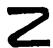
\includegraphics[keepaspectratio]{images/part001_8f5d44fd.jpg}}

\begin{enumerate}
\def\labelenumi{\arabic{enumi}.}
\setcounter{enumi}{4}
\tightlist
\item
  The logical framework of each chapter consists of the definitions, the axioms, and the theorems of the chapter. These are the parts that have mainly to be borne in mind for subsequent use. Less important results and those which can easily be deduced from the theorems are labelled as ``propositions,'' ``lemmas,'' ``corollaries,'' ``remarks,'' etc. Those which may be omitted at a first reading are printed in small type. A commentary on a particularly important theorem appears occasionally under the name of ``scholium.''
\end{enumerate}

To avoid tedious repetitions it is sometimes convenient to introduce notations or abbreviations which are in force only within a certain chapter or a certain section of a chapter (for example, in a chapter which is concerned only with commutative rings, the word ``ring'' would always signify ``commutative ring''). Such conventions are always explicitly mentioned, generally at the beginning of the chapter in which they occur.

\begin{enumerate}
\def\labelenumi{\arabic{enumi}.}
\setcounter{enumi}{5}
\tightlist
\item
  Some passages in the text are designed to forewarn the reader against serious errors. These passages are signposted in the margin with the sign
\end{enumerate}

Z (``dangerous bend'').

\begin{enumerate}
\def\labelenumi{\arabic{enumi}.}
\setcounter{enumi}{6}
\item
  The Exercises are designed both to enable the reader to satisfy himself that he has digested the text and to bring to his notice results which have no place in the text but which are nonetheless of interest. The most difficult exercises bear the sign ¶.
\item
  In general, we have adhered to the commonly accepted terminology, except where there appeared to be good reasons for deviating from it.
\item
  We have made a particular effort always to use rigorously correct language, without sacrificing simplicity. As far as possible we have drawn attention in the text to abuses of language, without which any mathematical text runs the risk of pedantry, not to say unreadability.
\item
  Since in principle the text consists of the dogmatic exposition of a theory, it contains in general no references to the literature. Bibliographical references are gathered together in Historical Notes, usually at the end of each chapter. These notes also contain indications, where appropriate, of the unsolved problems of the theory.
\end{enumerate}

The bibliography which follows each historical note contains in general only those books and original memoirs which have been of the greatest importance in the evolution of the theory under discussion. It makes no sort of pretence to completeness; in particular, references which serve only to determine questions of priority are almost always omitted.

As to the exercises, we have not thought it worthwhile in general to indicate their origins, since they have been taken from many different sources (original papers, textbooks, collections of exercises).

11. References to a part of this series are given as follows:\par

\begin{enumerate}
\def\labelenumi{\alph{enumi})}
\item
  If reference is made to theorems, axioms, or definitions presented in the same section, they are quoted by their number.
\item
  If they occur in another section of the same chapter, this section is also quoted in the reference.
\item
  If they occur in another chapter in the same Book, the chapter and section are quoted.
\item
  If they occur in another Book, this Book is first quoted by its title.
\end{enumerate}

The Summaries of Results are quoted by the letter R: thus Set Theory, R signifies ``Summary of Results of the Theory of Sets.''

\specialchapter{Contents of the Elements of Mathematics Series}

\textbf{I. THEORY OF SETS}\par

\begin{enumerate}
\def\labelenumi{\arabic{enumi}.}
\tightlist
\item
  Description of formal mathematics. 2. Theory of sets. 3. Ordered sets; cardinals; natural numbers. 4. Structures.
\end{enumerate}

\textbf{II. ALGEBRA}\par

\begin{enumerate}
\def\labelenumi{\arabic{enumi}.}
\tightlist
\item
  Algebraic structures. 2. Linear algebra. 3. Tensor algebras, exterior algebras, symmetric algebras. 4. Polynomials and rational fractions. 5. Fields. 6. Ordered groups and fields. 7. Modules over principal ideal rings. 8. Semi-simple modules and rings. 9. Sesquilinear and quadratic forms.
\end{enumerate}

\textbf{III. GENERAL TOPOLOGY}\par

\begin{enumerate}
\def\labelenumi{\arabic{enumi}.}
\tightlist
\item
  Topological structures. 2. Uniform structures. 3. Topological groups. 4. Real numbers. 5. One-parameter groups. 6. Real number spaces, affine and projective spaces. 7. The additive groups \(\mathbf{R}^n\) . 8. Complex numbers. 9. Use of real numbers in general topology. 10. Function spaces.
\end{enumerate}

\textbf{IV. FUNCTIONS OF A REAL VARIABLE}\par

\begin{enumerate}
\def\labelenumi{\arabic{enumi}.}
\tightlist
\item
  Derivatives. 2. Primitives and integrals. 3. Elementary functions. 4. Differential equations. 5. Local study of functions. 6. Generalized Taylor expansions. The Euler-Maclaurin summation formula. 7. The gamma function. Dictionary.
\end{enumerate}

\textbf{V. TOPOLOGICAL VECTOR SPACES}\par

\begin{enumerate}
\def\labelenumi{\arabic{enumi}.}
\tightlist
\item
  Topological vector spaces over a valued field. 2. Convex sets and locally convex spaces. 3. Spaces of continuous linear mappings. 4. Duality in topological vector spaces. 5. Hilbert spaces: elementary theory. Dictionary.
\end{enumerate}

\textbf{VI. INTEGRATION}\par

\begin{enumerate}
\def\labelenumi{\arabic{enumi}.}
\tightlist
\item
  Convexity inequalities. 2. Riesz spaces. 3. Measures on locally compact spaces. 4. Extension of a measure. L \(^{p}\) spaces. 5. Integration of measures. 6. Vectorial integration. 7. Haar measure. 8. Convolution and representation. 9. Integration on Hausdorff topological spaces.
\end{enumerate}


\textbf{LIE GROUPS AND LIE ALGEBRAS}\par

\begin{enumerate}
\def\labelenumi{\arabic{enumi}.}
\tightlist
\item
  Lie algebras. 2. Free Lie algebras. 3. Lie groups. 4. Coxeter groups and Tits systems. 5. Groups generated by reflections. 6. Root systems.
\end{enumerate}

\textbf{COMMUTATIVE ALGEBRA}\par

\begin{enumerate}
\def\labelenumi{\arabic{enumi}.}
\tightlist
\item
  Flat modules. 2. Localization. 3. Graduations, filtrations, and topologies. 4. Associated prime ideals and primary decomposition. 5. Integers. 6. Valuations. 7. Divisors.
\end{enumerate}

\textbf{SPECTRAL THEORIES}\par

\begin{enumerate}
\def\labelenumi{\arabic{enumi}.}
\tightlist
\item
  Normed algebras. 2. Locally compact groups.
\end{enumerate}

\textbf{DIFFERENTIABLE AND ANALYTIC MANIFOLDS}\par

Summary of results.

\specialchapter{Introduction}

The questions treated in this Book arose during the development of the theory of algebraic numbers and (later) algebraic geometry (cf.~the Historical Note). From the 19th century onwards these two theories began to show remarkable analogies; the attempt to solve the problems they posed led to the isolation of a number of general ideas whose field of application is not limited to rings of algebraic numbers or algebraic functions; and, as always, it is advantageous to consider these in their most general form in order to see their true significance and the repercussions of one study on another. The concepts treated in this Book can be applied in principle to all commutative rings and modules over such rings; it must however be pointed out that substantial results are often obtained only under certain hypotheses of finiteness (which always hold in the classical cases), for example by assuming the modules to be finitely generated or the rings to be Noetherian.

The chief notions central to the first chapters are the following:

I. Localization and globalization. Let us begin for example with a system of Diophantine equations:

\[
\mathrm{P} _ {i} (x _ {1}, \dots , x _ {m}) = 0 \quad (1 \leqslant i \leqslant n)\tag{*}
\]

where the \(P_{i}\) are polynomials with integer coefficients and solutions \((x_{i})\) are sought consisting of rational integers. It is possible to start approaching the problem by looking for solutions consisting of rational numbers, which involves looking at the same problem with the coefficients of the \(P_{i}\) considered as elements of the field of fractions Q of Z and the solutions sought with values in Q. A second step consists of seeing whether, given a prime number p, there exist rational solutions whose denominators are not divisible by p (integer solutions clearly satisfy this condition); this amounts, in this case, to lying in the subring \(\mathbf{Z}_{(p)}\) of Q consisting of the rational numbers of this form, called the local ring of Z corresponding to the prime number p.~Clearly the passage from Z to Q and that from Z to \(\mathbf{Z}_{(p)}\) are of the same form: in the two cases, the only denominators allowed do not belong to a certain prime ideal (the ideal (0) and the ideal (p) respectively). The same name ``local ring'' arises in algebraic geometry, where this notion appears in a more natural way: for example for the ring C{[}X{]} of polynomials in one variable with complex coefficients, the local ring corresponding to the prime ideal (X - \(\alpha\) ) is the ring of rational fractions ``regular'' at the point \(\alpha\) (that is, without a pole at that point).

Every Diophantine problem and more generally every problem on A-modules (A a commutative ring) can be decomposed into two subsidiary problems: its solution is sought in the local rings \(A_{p}\) corresponding to the different prime ideals p of A (``localization''), then the question is asked whether it is possible to conclude from the existence for all p of a solution to the ``localized'' problem that a solution exists to the problem posed initially (``passage from the local to the global''). Chapter II is devoted to the study of this double process and it is also seen that ``localization'' is not related only to prime ideals, but has a wider range.

\begin{enumerate}
\def\labelenumi{\Roman{enumi}.}
\setcounter{enumi}{1}
\tightlist
\item
  Completion of local rings. A local ring A shares with fields the property of having only one maximal ideal m. This fact is used to transform, to a certain extent, a problem on A-modules into an analogous problem on vector spaces by passing to the quotient ring A/m, as this latter is a field. If we return for example to the Diophantine system (*) this idea is none other than the principle of ``reduction modulo p'', transforming the equations into congruences mod. p, which occurred naturally beginning with the very first works in the theory of numbers.
\end{enumerate}

This being so, we clearly cannot hope in this way to obtain complete results for the original problem and it was quickly realized that to obtain more precise information it was necessary to consider, not only congruences modulo m, but also ``higher'' congruences modulo \(m^{n}\) , for arbitrary integers n \textgreater{} 0. It is thus found that, the larger n, the closer in some way the original problem is ``approached'' (in the case A = Z for example, the reason is that an integer \(\neq 0\) cannot be divisible by all the powers \(p^{n}\) of a given prime number p; this number will therefore make its presence felt in the reduction mod. \(p^{n}\) provided n is taken large enough). The mathematical translation of this idea consists of considering on A a ring topology (cf.~General Topology, Chapter III, § 6) in which the \(m^{n}\) form a fundamental system of neighbourhoods of 0. But when we have for example, solved the system of congruences

\[
\mathrm{P} _ {i} (x _ {1}, \dots , x _ {m}) \equiv 0 (\mathrm{mod.} p ^ {k}) \quad (1 \leqslant i \leqslant n)\tag{**}
\]

for every integer \(k > 0\) , it still does not follow that the system (*) has a solution in the local ring \(\mathbf{Z}_{(p)}\) ; the above hypothesis can be interpreted as saying that (*) admits a solution in the completion \(\hat{\mathbf{Z}}_{(p)}\) of the topological ring \(\mathbf{Z}_{(p)}\) .

The original problem, thus weakened, is finally transformed into the analogous problem for local rings of the type A/m \(^{n}\) , which are also nearer to fields
than general rings, since they have a nilpotent radical; in classical algebraic geometry this corresponds to a ``differential'' study of the problem in the neighbourhood of a given point.

Chapter III deals in a general way with these applications of topological notions to the theory of local rings. In Chapter VI a special aspect of this is studied, adapted on the one hand to more detailed studies of algebraic geometry, and above all to the arithmetic of algebraic number fields, where the local rings encountered (such as \(\mathbf{Z}_{(p)}\) ) belong to a particularly simple class, that of ``valuation rings'', where divisibility is a total ordering (cf.~Algebra, Chapter VI, §1) of the set of principal ideals.

The study of the passage from a ring A to a local ring \(A_{p}\) or to a completion \(\hat{A}\) brings to light a feature common to these two operations, the property of flatness of the A-modules \(A_{p}\) and \(\hat{A}\) , which allows amongst other things the use of tensor products of such A-modules with arbitrary A-modules somewhat similar to that of tensor products of vector spaces, that is, without all the precautions surrounding their use in the general case. The properties associated with this notion, which are also applicable to modules over non-commutative rings, are the object of study in Chapter I.

\begin{enumerate}
\def\labelenumi{\Roman{enumi}.}
\setcounter{enumi}{2}
\tightlist
\item
  Integers and decomposition of ideals. The study of divisibility in algebraic number fields necessitated from the start the introduction of the notion of integer in such a field K, generalizing the notion of rational integer in the field Q. The general theory of this notion of ``algebraic integer'', linked, as will be seen, to very strict conditions of finiteness, is developed in Chapter V; it can be applied to all commutative rings and is of great interest not only in arithmetic, but in algebraic geometry and even in the modern theory of ``analytic spaces'' over the field C.
\end{enumerate}

One of the major obstacles to the extension of classical arithmetic to rings of algebraic integers has long been that the classical decomposition of a rational integer into prime factors does not extend in general to these rings. The creation of the theory of ideals was necessary to surmount this difficulty: the unique decomposition sought is then established for ideals, the notion of prime ideal being substituted for that of prime number. Moreover this result can be considered as a typical case where the ``passage from the local to the global'' is performed satisfactorily: the knowledge, for \(x \in K\) , of the values at x of all the ``valuations'' on K determines x up to multiplication by an invertible integer.

In less simple rings than rings of algebraic integers (and even for example in rings of polynomials in several indeterminates) this result is no longer valid. However it is possible to associate in a canonical way with every ideal a well-determined set of prime ideals: in algebraic geometry, if we consider for example in \(K^{n}\) (K any commutative field) a subvariety defined by a system of polynomial equations \(P_{\alpha}=0\) , the irreducible components of this subvariety correspond bijectively with the minimal elements of the set of prime ideals thus associated with the ideal generated by the \(P_{\alpha}\) . It is moreover possible (if we restrict ourselves to Noetherian rings) to give for every ideal a ``decomposition'' less precise than a decomposition as a product of prime ideals: here the product is in fact replaced by the intersection and the powers of prime ideals by ``primary'' ideals connected with the prime ideals associated with the ideal in question (but which are not direct generalizations of powers of prime ideals). The introduction of prime ideals associated with an ideal and the study of their properties is the subject of Chapter IV; here also the existence and certain uniqueness properties of the ``primary decompositions'' to which we have just alluded are proved; but it seems at present that these decompositions usually only play an accessory role in applications, the essential notion being that of prime ideal associated with an ideal.

In Chapter VII we examine in more detail rings whose properties most nearly approach those of rings of algebraic integers as far as decomposition as a product of prime ideals is concerned; amongst other things it is possible to introduce into these rings the notion of ``divisor'', which is the geometric aspect of this decomposition and plays an important role in algebraic geometry.

Finally Chapters VIII et seq. will deal with notions of more interest in algebraic geometry than in arithmetic (where they become trivial) and notably the concept of dimension.

With these notions we come to the frontier of algebraic geometry proper, a frontier which is ever moving and difficult to trace. For, if commutative algebra is an essential tool for the development of algebraic geometry in all its generality, conversely (as has already been seen above) the language of geometry proves very convenient for expressing the theorems of commutative algebra and suggesting a certain intuition naturally enough absent from abstract algebra; with the tendency to enlarge more and more the limits of algebraic geometry, algebraic and geometric language tend more than ever to merge.

CHAPTER I(*)

\chapter{Flat Modules}

Unless otherwise stated, all the rings considered in this chapter are assumed to have a unit element; all the ring homomorphisms are assumed to map unit element to unit element. A subring of a ring A means a subring containing the unit element of A.

If A is a ring, M a left A-module and U (resp. V) an additive subgroup of A (resp. M), recall that UV or U. V is used to denote the additive subgroup of M generated by the products uv, where \(u \in U\) , \(v \in V\) (Algebra, Chapter VIII, § 6, no. 1). If a is an ideal of A, we write \(a^{0} = A\) . For any set E, \(1_{E}\) (or 1 if no confusion arises) is used to denote the identity mapping of E to itself.

Recall that the axioms for a module imply that if E is a left (resp. right) module over a ring A and 1 denotes the unit element of A, then 1.x = x (resp. x.1 = x) for all \(x \in E\) (Algebra, Chapter II, §1, no. 1). If E and F are two left (resp. right) A-modules, recall that \(\operatorname{Hom}_{\mathbf{A}}(\mathbf{E}, \mathbf{F})\) (or simply \(\operatorname{Hom}(\mathbf{E}, \mathbf{F})\) ) is used to denote the additive group of homomorphisms of E to F (loc. cit., §1, no. 2). By an abuse of notation 0 will often be used to denote a module reduced to its identity element.

\section{DIAGRAMS AND EXACT SEQUENCES}

\subsection{Diagrams}

Let, for example, A, B, C, D, E be five sets and let f be a mapping from A to B, g a mapping from B to C, h a mapping from D to E, u a mapping from B to D and v a mapping from C to E. To summarize such a situation we often make use of diagrams; for example, the above situation is summarized by the following diagram (Set Theory, Chapter II, § 3, no. 4):

\begin{enumerate}
\def\labelenumi{(\arabic{enumi})}
\tightlist
\item
\end{enumerate}

\pandocbounded{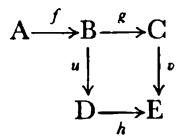
\includegraphics[keepaspectratio]{images/part001_a608eb63.jpg}}

In such a diagram the group of symbols A \(\xrightarrow{f}\) B expresses schematically the fact that f is a mapping from A to B. Where there is no ambiguity about f, we suppress the letter f and write simply A \(\rightarrow\) B.

When A, B, C, D, E are groups (resp. commutative groups) and f, g, h, u, v group homomorphisms, diagram (1) is called, by way of abbreviation, a diagram of groups (resp. commutative groups).

In principle, a diagram is not a mathematical object, but only a figure designed to facilitate reading an argument. In practice, diagrams are often used as abbreviatory symbols to avoid naming all the sets and mappings under consideration; we therefore say ``Consider the diagram (1)'' instead of saying ``Let A, B, C, D, E be five sets . . . and v a mapping from C to E''; see for example the statement of Proposition 2 in no. 4.

\subsection{Commutative diagrams}

Consider, for example, the following diagram:

\[
\begin{array}{c} \mathrm{A} \xrightarrow {f} \mathrm{B} \xrightarrow {g} \mathrm{C} \xrightarrow {h} \mathrm{D} \\ a \Big \downarrow \qquad b \Big \downarrow \qquad c \Big \downarrow \qquad d \Big \downarrow \\ \mathrm{A} ^ {\prime} \xrightarrow [ f ^ {\prime} ]{} \mathrm{B} ^ {\prime} \xrightarrow [ g ^ {\prime} ]{} \mathrm{C} ^ {\prime} \xrightarrow [ h ^ {\prime} ]{} \mathrm{D} ^ {\prime} \end{array}\tag{2}
\]

To every path composed of a certain number of segments of the diagram traversed in the direction shown by the arrows corresponds a mapping of the set represented by the beginning of the first segment to the set represented by the end of the last segment, namely the composition of the mappings represented by the various segments traversed. For each vertex of the diagram, for example B, by way of convention there is a path reduced to B, to which corresponds the identity mapping \(l_{B}\) .

In (2) there are for example three paths beginning at A and ending at C'; the corresponding mappings are \(c \circ g \circ f\) , \(g' \circ b \circ f\) and \(g' \circ f' \circ a\) . A diagram is said to be commutative if, for every pair of paths in the diagram with the same beginning and end, the two corresponding mappings are equal; in particular if the beginning and end of a path coincide the corresponding mapping must be the identity.

For the diagram (2) to be commutative it is necessary and sufficient that the relations

\[
f ^ {\prime} \circ a = b \circ f, \quad g ^ {\prime} \circ b = c \circ g, \quad h ^ {\prime} \circ f = d \circ h;\tag{3}
\]

hold; in other words, it is necessary and sufficient that the three square diagrams contained in (2) be commutative. For the relations (3) imply \(c \circ g \circ f = g' \circ b \circ f\) since \(c \circ g = g' \circ b\) , and \(g' \circ b \circ f = g' \circ f' \circ a\) since \(b \circ f = f' \circ a\) ; thus the three paths beginning at A and ending at C' give the same mapping. It can be similarly verified that the four paths beginning at A and ending at D' (resp. the three paths beginning at B and ending at D') give the same mapping. The relations (3) signify that the two paths beginning at A (resp. B, C) and ending at B' (resp. C', D') give the same mapping. None of the other pairs of vertices of (2) can be joined by more than one path and the diagram (2) is therefore commutative.

In what follows we shall leave the reader to verify analogous results for other types of diagrams.

\subsection{Exact sequences}

Recall the following definition (Algebra, Chapter II, § 1, no. 4):

DEFINITION 1. Let A be a ring, F, G, H three right (resp. left) A-modules, f a homomorphism of F to G and g a homomorphism of G to H. The ordered pair \((f, g)\) is called an exact sequence if \(\bar{g}^{-1}(0) = f(F)\) , that is if the kernel of g is equal to the image of f.

The diagram

\[
\mathrm{F} \xrightarrow {f} \mathrm{G} \xrightarrow {g} \mathrm{H}\tag{4}
\]

is also called an exact sequence.

Consider similarly a diagram consisting of four modules and three homomorphisms:

\[
\mathrm{E} \xrightarrow {f} \mathrm{F} \xrightarrow {g} \mathrm{G} \xrightarrow {h} \mathrm{H}.\tag{5}
\]

This diagram is said to be exact at F if the diagram \(E \xrightarrow{f} F \xrightarrow{g} G\) is an exact sequence; it is said to be exact at G if \(F \xrightarrow{g} G \xrightarrow{h} H\) is an exact sequence. If (5) is exact at F and G, it is said to be exact or also an exact sequence. Exact sequences with any number of terms are similarly defined.

Recall the following results (loc. cit.), where E, F, G denote right (resp. left)

A-modules, the arrows represent homomorphisms and 0 denotes a module reduced to its identity element:

\begin{enumerate}
\def\labelenumi{(\alph{enumi})}
\item
  To say that \(0 \to \mathbf{E} \xrightarrow{f} \mathbf{F}\) is an exact sequence is equivalent to saying that \(f\) is injective.
\item
  To say that \(\mathbf{E} \xrightarrow{f} \mathbf{F} \to 0\) is an exact sequence is equivalent to saying that \(f\) is surjective.
\item
  To say that \(0 \to \mathbf{E} \xrightarrow{f} \mathbf{F} \to 0\) is an exact sequence is equivalent to saying that \(f\) is bijective, that is that \(f\) is an isomorphism of \(\mathbf{E}\) onto \(\mathbf{F}\) .
\item
  If F is a submodule of E and i denotes the canonical injection of F into E and p the canonical surjection of E onto E/F, the diagram
\end{enumerate}

\[
0 \longrightarrow \mathrm{F} \stackrel {i} {\longrightarrow} \mathrm{E} \stackrel {p} {\longrightarrow} \mathrm{E} / \mathrm{F} \longrightarrow 0\tag{6}
\]

is an exact sequence.

\begin{enumerate}
\def\labelenumi{(\alph{enumi})}
\setcounter{enumi}{4}
\tightlist
\item
  If \(f: \mathbf{E} \to \mathbf{F}\) is a homomorphism, the diagram
\end{enumerate}

\[
0 \longrightarrow \overline {{f}} ^ {- 1} (0) \stackrel {i} {\longrightarrow} \mathrm{E} \stackrel {f} {\longrightarrow} \mathrm{F} \stackrel {p} {\longrightarrow} \mathrm{F} / f (\mathrm{E}) \longrightarrow 0\tag{7}
\]

(where \(i\) is the canonical injection of \(\overline{f}(0)\) into E and \(p\) the canonical projection of \(\mathbf{F} / f(\mathbf{E})\) ) is an exact sequence.

\begin{enumerate}
\def\labelenumi{(\alph{enumi})}
\setcounter{enumi}{5}
\tightlist
\item
  For the diagram
\end{enumerate}

\[
\mathrm{E} \xrightarrow {f} \mathrm{F} \xrightarrow {g} \mathrm{G}\tag{8}
\]

to be an exact sequence, it is necessary and sufficient that there exist modules S, T and homomorphisms \(a: \mathrm{E} \to \mathrm{S}\) , \(b: \mathrm{S} \to \mathrm{F}\) , \(c: \mathrm{F} \to \mathrm{T}\) and \(d: \mathrm{T} \to \mathrm{G}\) such that \(f = b \circ a\) , \(g = d \circ c\) and the three sequences

\[
\begin{array}{c} \mathrm{E} \xrightarrow {a} \mathrm{S} \longrightarrow 0 \\ 0 \longrightarrow \mathrm{S} \xrightarrow {b} \mathrm{F} \xrightarrow {c} \mathrm{T} \longrightarrow 0 \\ 0 \longrightarrow \mathrm{T} \xrightarrow {d} \mathrm{G} \end{array}\tag{9}
\]

be exact.

Recall finally that if \(f: \mathbf{E} \to \mathbf{F}\) is an A-module homomorphism, we set \(\operatorname{Ker}(f) = \bar{f}^{-1}(0)\) , \(\operatorname{Im}(f) = f(\mathbf{E})\) , \(\operatorname{Coim}(f) = \mathbf{E} / \bar{f}^{-1}(0)\) and \(\operatorname{Coker}(f) = \mathbf{F} / f(\mathbf{E})\) . With this notation it is possible to take, in (9), \(\mathbf{S} = \operatorname{Im}(f) = \operatorname{Ker}(g)\) and \(\mathbf{T} = \operatorname{Im}(g)\) (canonically isomorphic to \(\operatorname{Coker}(f)\) ).

\subsection{The snake diagram}

PROPOSITION 1. Consider a commutative diagram of commutative groups:

\[
\begin{array}{c c c} \mathrm{A} & \xrightarrow {u} & \mathrm{B} \\ a \Big \downarrow & & b \Big \downarrow \\ \mathrm{A} ^ {\prime} & \xrightarrow {} u ^ {\prime} & \mathrm{B} ^ {\prime} \end{array} \xrightarrow {v} \begin{array}{c c c} \mathrm{C} \\ c \Big \downarrow \\ \mathrm{C} ^ {\prime} \end{array}\tag{10}
\]

Suppose that the two rows of (10) are exact. Then:

\begin{enumerate}
\def\labelenumi{(\roman{enumi})}
\tightlist
\item
  If \(c\) is injective, we have
\end{enumerate}

\[
\operatorname{Im} (b) \cap \operatorname{Im} (u ^ {\prime}) = \operatorname{Im} (u ^ {\prime} \circ a) = \operatorname{Im} (b \circ u).\tag{11}
\]

\begin{enumerate}
\def\labelenumi{(\roman{enumi})}
\setcounter{enumi}{1}
\tightlist
\item
  If \(a\) is surjective, we have
\end{enumerate}

\[
\operatorname{Ker} (b) \dot {+} \operatorname{Im} (u) = \operatorname{Ker} (v ^ {\prime} \circ b) = \operatorname{Ker} (c \circ v).\tag{12}
\]

Let us prove (i). Clearly

\[
\operatorname{Im} (u ^ {\prime} \circ a) = \operatorname{Im} (b \circ u) \subset \operatorname{Im} (b) \cap \operatorname{Im} (u ^ {\prime}).
\]

Conversely, let \(x \in \operatorname{Im}(b) \cap \operatorname{Im}(u')\) . There exists \(y \in B\) such that \(x = b(y)\) . As \(v' \circ u' = 0\) , we have \(0 = v'(x) = v'(b(y)) = c(v(y))\) , whence \(v(y) = 0\) since \(c\) is injective. As \((u, v)\) is an exact sequence, there exists \(z \in A\) such that \(y = u(z)\) , whence \(x = b(u(z))\) .

Let us prove (ii). As \(v \circ u = 0\) and \(v' \circ u' = 0\) , it is clear that

\[
\operatorname{Ker} (b) + \operatorname{Im} (u) \subset \operatorname{Ker} (v ^ {\prime} \circ b) = \operatorname{Ker} (c \circ v).
\]

Conversely, let \(x \in \operatorname{Ker}(v' \circ b)\) . Then \(b(x) \in \operatorname{Ker}(v')\) and there exists \(y' \in A'\) such that \(u'(y') = b(x)\) , since the sequence \((u', v')\) is exact. As \(a\) is surjective, there exists \(y \in A\) such that \(a(y) = y'\) , whence \(b(x) = u'(a(y)) = b(u(y))\) ; it follows that \(x - u(y) \in \operatorname{Ker}(b)\) , which completes the proof.

LEMMA 1. Consider a commutative diagram of commutative groups:

\[
\begin{array}{c} \mathrm{A} \xrightarrow {u} \mathrm{B} \\ a \Big \downarrow \\ \mathrm{A} ^ {\prime} \xrightarrow [ u ^ {\prime} ]{} \mathrm{B} ^ {\prime} \end{array}\tag{13}
\]

Then there exists one and only one homomorphism \(u_1 \colon \operatorname{Ker}(a) \to \operatorname{Ker}(b)\) and one and only one homomorphism \(u_2 \colon \operatorname{Coker}(a) \to \operatorname{Coker}(b)\) such that the diagrams

\begin{enumerate}
\def\labelenumi{(\arabic{enumi})}
\setcounter{enumi}{13}
\tightlist
\item
\end{enumerate}

and

\pandocbounded{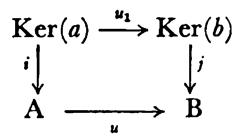
\includegraphics[keepaspectratio]{images/part001_d47c3bb2.jpg}}

\begin{enumerate}
\def\labelenumi{(\arabic{enumi})}
\setcounter{enumi}{14}
\tightlist
\item
\end{enumerate}

\pandocbounded{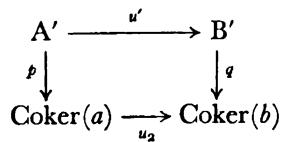
\includegraphics[keepaspectratio]{images/part001_9d56bddd.jpg}}

are commutative, \(i\) and \(j\) denoting the canonical injections and \(p\) and \(q\) the canonical surjections.

If \(x \in \operatorname{Ker}(a)\) , then \(a(x) = 0\) and \(b(u(x)) = u'(a(x)) = 0\) , hence \(u(x) \in \operatorname{Ker}(b)\) , and the existence and uniqueness of \(u_1\) are then immediate. Similarly, we have \(u'(a(A)) = b(u(A)) \subset b(B)\) , then by taking quotients \(u'\) gives a homomorphism \(u_2\) : \(\operatorname{Coker}(a) \to \operatorname{Coker}(b)\) , which is the only homomorphism for which (15) is commutative.

Let us now start with the commutative diagram (10) of commutative groups; there corresponds to it by Lemma 1 a diagram

\begin{enumerate}
\def\labelenumi{(\arabic{enumi})}
\setcounter{enumi}{15}
\tightlist
\item
\end{enumerate}

\pandocbounded{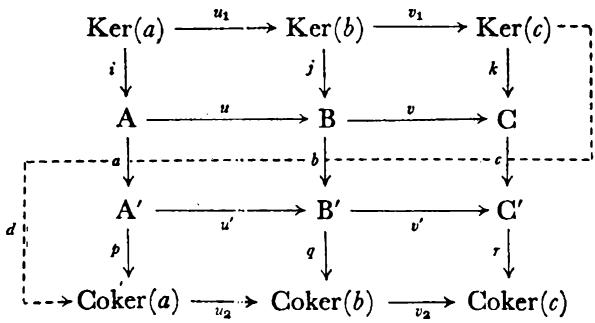
\includegraphics[keepaspectratio]{images/part001_af6ee28a.jpg}}

where \(i, j, k\) are the canonical injections, \(p, q, r\) the canonical surjections and \(u_{1}, u_{2}\) (resp. \(v_{1}, v_{2}\) ) the homomorphisms canonically associated with \(u, u'\) (resp. \(v, v'\) ) by Lemma 1. It is immediately verified that this diagram is commutative.

PROPOSITION 2. Suppose that in the commutative diagram (10) the sequences \((u, v)\) and \((u', v')\) are exact. Then:

\begin{enumerate}
\def\labelenumi{(\roman{enumi})}
\item
  \(v_{1} \circ u_{1} = 0\) ; if \(u'\) is injective, the sequence \((u_{1}, v_{1})\) is exact.
\item
  \(v_{2} \circ u_{2} = 0\) ; if \(v\) is surjective, the sequence \((u_{2}, v_{2})\) is exact.
\item
  Suppose that \(u'\) is injective and \(v\) is surjective. Then there exists one and only one homomorphism \(d: \operatorname{Ker}(c) \to \operatorname{Coker}(a)\) with the following property: if \(x \in \operatorname{Ker}(c)\) , \(y \in B\) and \(t' \in A'\) satisfy the relations \(v(y) = k(x)\) and \(u'(t') = b(y)\) , then \(d(x) = p(t')\) . Moreover the sequence
\end{enumerate}

\[
(*) \quad \operatorname{Ker} (a) \xrightarrow {u _ {1}} \operatorname{Ker} (b) \xrightarrow {v _ {1}} \operatorname{Ker} (c) \xrightarrow {d}
\]

\[
\operatorname{Coker} (a) \xrightarrow {u _ {2}} \operatorname{Coker} (b) \xrightarrow {v _ {2}} \operatorname{Coker} (c)
\]

is exact.

Let us prove (i). As \(u_{1}\) and \(v_{1}\) have the same graphs as the restrictions of \(u\) and \(v\) to \(\operatorname{Ker}(a)\) and \(\operatorname{Ker}(b)\) respectively, we have \(v_{1} \circ u_{1} = 0\) . Then

\[
\operatorname{Ker} (v _ {1}) = \operatorname{Ker} (b) \cap \operatorname{Ker} (v) = \operatorname{Ker} (b) \cap \operatorname{Im} (u) = \operatorname{Im} (j) \cap \operatorname{Im} (u).
\]

But, by Proposition 1, (i), \(\operatorname{Ker}(v_1) = \operatorname{Im}(j \circ u_1) = \operatorname{Im}(u_1)\) if \(u'\) is injective.

Let us prove (ii). As \(u_{2}\) and \(v_{2}\) are obtained from \(u\) and \(v\) by taking quotients, it is clear that \(v_{2} \circ u_{2} = 0\) . Suppose that \(v\) is surjective; as \(q\) and \(p\) are surjective, it follows from the hypotheses and Proposition 1, (ii) that

\[
\begin{array}{r l} \operatorname{Ker} (v _ {2}) & = q (\operatorname{Ker} (v _ {2} \circ q)) = q (\operatorname{Ker} (v ^ {\prime}) + \operatorname{Im} (b)) = q (\operatorname{Ker} (v ^ {\prime})) = q (\operatorname{Im} (u ^ {\prime})) \\ & = \operatorname{Im} (q \circ u ^ {\prime}) = \operatorname{Im} (u _ {2} \circ p) = \operatorname{Im} (u _ {2}). \end{array}
\]

Finally let us prove (iii). For \(x \in \operatorname{Ker}(c)\) there exists \(y \in B\) such that \(v(y) = k(x)\) since \(v\) is surjective; moreover \(v'(b(y)) = c(k(x)) = 0\) and consequently there exists a unique \(t' \in A'\) such that \(u'(t') = b(y)\) , since \(u'\) is injective. We now show that the element \(p(t') \in \operatorname{Coker}(a)\) is independent of the element \(y \in B\) such that \(v(y) = k(x)\) . For if \(y' \in B\) is another element such that \(v(y') = k(x)\) , then \(y' = y + u(z)\) , where \(z \in A\) ; we show that if \(t'' \in A'\) is such that \(u'(t'') = b(y')\) then \(t'' = t' + a(z)\) ; for

\[
u ^ {\prime} \left(t ^ {\prime} + a (z)\right) = u ^ {\prime} \left(t ^ {\prime}\right) + u ^ {\prime} (a (z)) = b (y) + b (u (z)) = b (y + u (z)) = b \left(y ^ {\prime}\right).
\]

Finally, it follows that \(p(t'') = p(t') + p(a(z)) = p(t')\) . Then it is possible to set \(d(x) = p(t')\) and the mapping \(d: \operatorname{Ker}(c) \to \operatorname{Coker}(a)\) has thus been defined. If now \(x_1, x_2\) are elements of \(\operatorname{Ker}(c)\) and \(x = x_1 + x_2\) , we take elements \(y_1, y_2\) of B such that \(v(y_1) = k(x_1)\) and \(v(y_2) = k(x_2)\) and choose for \(y \in B\) the element \(y_1 + y_2\) ; it is then immediate that \(d(x) = d(x_1) + d(x_2)\) and hence \(d\) is a homomorphism.

Suppose that \(x = v_{1}(x')\) for some \(x' \in \operatorname{Ker}(b)\) ; then take \(y \in B\) to be the element \(j(x')\) . As \(b(j(x')) = 0\) , it follows that \(d(x) = 0\) , hence \(d \circ v_{1} = 0\) . Conversely, suppose that \(d(x) = 0\) . In the above notation we then have \(t' = a(s)\) , where \(s \in A\) . In this case we have \(b(y) = u'(t') = u'(a(s)) = b(u(s))\) , or \(b(y - u(s)) = 0\) . The element \(y - u(s)\) is therefore of the form \(j(n)\) , where \(n \in \operatorname{Ker}(b)\) , and we have \(k(x) = v(y) = v(u(s) + j(n)) = v(j(n)) = k(v_1(n))\) ; as \(k\) is injective, \(x = v_1(n)\) , which proves that the sequence (*) is exact at \(\operatorname{Ker}(c)\) .

Finally, we have (always in the same notation)

\[
u _ {2} (d (x)) = u _ {2} \left(p \left(t ^ {\prime}\right)\right) = q \left(u ^ {\prime} \left(t ^ {\prime}\right)\right) = q (b (y)) = 0
\]

and hence \(u_2 \circ d = 0\) . Conversely, suppose that an element \(w = p(t')\) of Coker(a) is such that \(u_2(w) = u_2(p(t')) = 0\) (where \(t' \in A'\) ). Then \(q(u'(t')) = 0\) and consequently \(u'(t') = b(y)\) for some \(y \in B\) ; as \(v'(u'(t')) = 0\) , we have \(v'(b(y)) = 0\) , hence \(c(v(y)) = 0\) , in other words \(v(y) = k(x)\) for some \(x \in \operatorname{Ker}(c)\) , and by definition \(w = d(x)\) , which shows that the sequence (*) is exact at

Coker(a). It has been seen in (i) that it is exact at \(\operatorname{Ker}(b)\) and in (ii) it is exact at \(\operatorname{Coker}(b)\) , which completes the proof of (iii).

Remark. If the groups of the diagram (10) are all (for example, right) modules over a ring \(\Lambda\) and the homomorphisms are \(\Lambda\) -module homomorphisms, it is soon verified that the homomorphism \(d\) defined in Proposition 2, (iii) is also a \(\Lambda\) -module homomorphism: if \(x \in \operatorname{Ker}(c)\) and \(\alpha \in \Lambda\) , and \(y \in B\) is such that \(v(y) = k(x)\) , it is sufficient to note that \(v(y\alpha) = k(x\alpha)\) .

COROLLARY 1. Suppose that the diagram (10) is commutative and the two rows are exact. Then:

\begin{enumerate}
\def\labelenumi{(\roman{enumi})}
\item
  If \(u'\) , \(a\) and \(c\) are injective, \(b\) is injective.
\item
  If \(v, a\) and \(c\) are surjective, \(b\) is surjective.
\end{enumerate}

Assertion (i) is a consequence of assertion (i) of Proposition 2: for \(\operatorname{Ker}(a) = 0\) and \(\operatorname{Ker}(c) = 0\) , hence \(\operatorname{Ker}(b) = 0\) .

Assertion (ii) is a consequence of assertion (ii) of Proposition 2: for \(\operatorname{Coker}(a) = 0\) and \(\operatorname{Coker}(c) = 0\) , hence \(\operatorname{Coker}(b) = 0\) .

COROLLARY 2. Suppose that the diagram (10) is commutative and the two rows are exact. Under these conditions:

\begin{enumerate}
\def\labelenumi{(\roman{enumi})}
\item
  If \(b\) is injective and if \(a\) and \(v\) are surjective, then \(c\) is injective.
\item
  If \(b\) is surjective and if \(c\) and \(u'\) are injective, then \(a\) is surjective.
\end{enumerate}

To prove (i) consider the diagram

\[
\begin{array}{c c c} u (\mathrm{A}) & \xrightarrow {w} \mathrm{B} & \xrightarrow {v} \mathrm{C} \\ a ^ {\prime} \Big \downarrow & b \Big \downarrow & c \Big \downarrow \\ u ^ {\prime} (\mathrm{A} ^ {\prime}) & \xrightarrow [ w ^ {\prime} ]{} \mathrm{B} ^ {\prime} & \xrightarrow [ v ^ {\prime} ]{} \mathrm{C} ^ {\prime} \end{array}
\]

where \(a'\) is the mapping with the same graph as the restriction of b to \(u(\mathbf{A})\) and w and \(w'\) are the canonical injections; clearly this diagram is commutative and its rows exact. Moreover \(w'\) is injective and by hypothesis v is surjective; then by Proposition 2, (iii) we have an exact sequence

\[
0 = \operatorname{Ker} (b) \longrightarrow \operatorname{Ker} (c) \stackrel {d} {\longrightarrow} \operatorname{Coker} (a ^ {\prime}) = 0
\]

since \(b\) is injective and \(a'\) is surjective; whence \(\operatorname{Ker}(c) = 0\) .

To prove (ii) consider the diagram

\[
\begin{array}{c} \mathrm{A} \xrightarrow {u} \mathrm{B} \xrightarrow {w} v (\mathrm{B}) \\ a ^ {\prime} \Biggl \downarrow \qquad \qquad b \Biggl \downarrow \qquad \qquad c ^ {\prime} \Biggl \downarrow \\ \mathrm{A} ^ {\prime} \xrightarrow [ w ^ {\prime} ]{} \mathrm{B} ^ {\prime} \xrightarrow [ v ^ {\prime} ]{} v ^ {\prime} (\mathrm{B} ^ {\prime}) \end{array}
\]

where this time \(c'\) is the mapping with the same graph as the restriction of c to \(v(\mathbf{B})\) and \(w\) and \(w'\) have respectively the same graphs as \(v\) and \(v'\) ; this diagram is commutative and its rows exact. Moreover \(w\) is surjective and by hypothesis \(u'\) is injective; then by Proposition 2, (iii) we have an exact sequence

\[
0 = \operatorname{Ker} (c ^ {\prime}) \xrightarrow {d} \operatorname{Coker} (a) \longrightarrow \operatorname{Coker} (b) = 0
\]

since \(b\) is surjective and \(c'\) is injective; whence Coker \((a) = 0\) .

\section{FLAT MODULES}

\subsection{Revision of tensor products}

Let A be a ring, E a right A-module and M a left A-module. In Algebra, Chapter II, §3, no. 1 we defined the tensor product \(\mathbf{E} \otimes_{\mathbf{A}} \mathbf{M}\) , which is a \(\mathbf{Z}\) -module. If \(\mathbf{E}'\) (resp. \(\mathbf{M}'\) ) is a right (resp. left) A-module and \(u: \mathbf{E} \to \mathbf{E}'\) (resp. \(v: \mathbf{M} \to \mathbf{M}'\) ) a homomorphism, we also defined (loc. cit, no. 2) a \(\mathbf{Z}\) -homomorphism

\[
\boldsymbol {u} \otimes v: \mathrm{E} \otimes_ {\mathrm{A}} \mathrm{M} \rightarrow \mathrm{E} ^ {\prime} \otimes_ {\mathrm{A}} \mathrm{M} ^ {\prime}.
\]

LEMMA 1. Let \(\mathbf{M}' \xrightarrow{v} \mathbf{M} \xrightarrow{w} \mathbf{M}'' \to 0\) be an exact sequence of left A-modules and E a right A-module. Then the sequence

\[
\mathrm{E} \otimes_ {\mathrm{A}} \mathrm{M} ^ {\prime} \xrightarrow {1 \otimes v} \mathrm{E} \otimes_ {\mathrm{A}} \mathrm{M} \xrightarrow {1 \otimes w} \mathrm{E} \otimes_ {\mathrm{A}} \mathrm{M} ^ {\prime \prime} \longrightarrow 0
\]

is an exact sequence of commutative groups.

This is the Corollary to Proposition 5 of Algebra, Chapter II, § 3, no. 6.

It follows that, for any left A-module homomorphism \(u: M \rightarrow N\) ,

\[
\mathrm{E} \otimes_ {\mathbf {A}} (\text { Coker } u)
\]

is canonically identified with \(\operatorname{Coker}(1_{E} \otimes u)\) , as Lemma 1 shows when applied to the exact sequence

\[
\mathrm{M} \xrightarrow {u} \mathrm{N} \longrightarrow \text { Coker } u \longrightarrow 0.
\]

In the notation of Lemma 1, we know (loc. cit.) that if v is injective, that is if the sequence \(0 \rightarrow M' \stackrel{v}{\rightarrow} M \stackrel{w}{\rightarrow} M'' \rightarrow 0\) is exact, it does not necessarily follow that \(1_{E} \otimes v\) is injective and so \(E \otimes_{A} M'\) cannot in general be identified with a subgroup of E \(\otimes_{\mathbf{A}}\) M. Recall however (Algebra, Chapter II, § 3, no. 7, Corollary 5 to Proposition 7) the following result:

LEMMA 2. If \(v: \mathbf{M}' \to \mathbf{M}\) is injective and \(v(\mathbf{M}')\) is a direct factor of \(\mathbf{M}\) , the homomorphism \(1_{\mathbf{E}} \otimes v\) is injective and its image is a direct factor of \(\mathbf{E} \otimes_{\mathbf{A}} \mathbf{M}\) .

\subsection{M-flat modules}

DEFINITION 1. Let A be a ring, E a right A-module and M a left A-module. E is said to be flat for M (or M-flat) if, for every left A-module M' and every injective homomorphism \(v: M' \to M\), the homomorphism \(1_{E} \otimes v\) : E \(\otimes_{A} M' \to E \otimes_{A} M\) is injective.

For any right A-module N, the notion of an N-flat left module is defined similarly. To say that a right A-module E is flat for a left A-module M is equivalent to saying that E, considered as a left \(A^{0}\) -module (recall that \(A^{0}\) denotes the opposite ring to A), is flat for the right \(A^{0}\) -module M.

LEMMA 3. For a right A-module E to be M-flat, it is necessary and sufficient that for every finitely generated submodule M' of M the canonical homomorphism

\[
\mathbf {1} _ {\mathbf {E}} \otimes j: \mathbf {E} \otimes_ {\mathbf {A}} \mathbf {M} ^ {\prime} \rightarrow \mathbf {E} \otimes_ {\mathbf {A}} \mathbf {M}
\]

(j being the canonical injection \(\mathbf{M}'\to \mathbf{M}\) ) be injective.

Suppose that this condition holds and let N be any submodule of M. Suppose that the canonical image in \(E \otimes_{A} M\) of an element

\[
z = \sum_ {i} x _ {i} \otimes y _ {i} \in \mathbf {E} \otimes_ {\mathbf {A}} \mathbf {N} (x _ {i} \in \mathbf {E}, y _ {i} \in \mathbf {N})
\]

is zero and let \(M'\) be the finitely generated submodule of N generated by the \(y_{i}\) ; as by hypothesis the composite mapping \(E \otimes_{A} M' \to E \otimes_{A} N \to E \otimes_{A} M\) is injective, the sum \(z' = \sum_{i} x_{i} \otimes y_{i}\) , considered as an element of \(E \otimes_{A} M'\) , is zero. As z is the image of \(z'\) , we have also z = 0, whence the lemma.

LEMMA 4. Let E be a right A-module and M a left A-module such that E is M-flat. If N is either a submodule or a quotient module of M, then E is N-flat.

The case in which N is a submodule is easy, as, if \(N'\) is a submodule of N, the composite homomorphism

\[
\mathrm{E} \otimes_ {\mathrm{A}} \mathrm{N} ^ {\prime} \rightarrow \mathrm{E} \otimes_ {\mathrm{A}} \mathrm{N} \rightarrow \mathrm{E} \otimes_ {\mathrm{A}} \mathrm{M}
\]

is injective, hence so is \(\mathbf{E} \otimes_{\mathbf{A}} \mathbf{N}' \to \mathbf{E} \otimes_{\mathbf{A}} \mathbf{N}\) . Suppose then that \(\mathbf{N}\) is a quotient module of \(\mathbf{M}\) , that is there exists an exact sequence \(0 \to \mathbf{R} \xrightarrow{i} \mathbf{M} \xrightarrow{p} \mathbf{N} \to 0\) . Let \(\mathbf{N}'\) be a submodule of \(\mathbf{N}\) and \(\mathbf{M}' = \bar{p}^{-1}(\mathbf{N}')\) . Let \(i'\) denote the mapping of \(\mathbf{R}\) to \(\mathbf{M}'\) with the same graph as \(i, p'\) the surjection \(\mathbf{M}' \to \mathbf{N}'\) with the same graph as the restriction of \(p\) to \(\mathbf{M}'\) , \(r\) the identity mapping of \(\mathbf{R}\) to \(\mathbf{R}\) , \(m\) the canonical injection \(\mathbf{M}' \to \mathbf{M}\) and \(n\) the canonical injection \(\mathbf{N}' \to \mathbf{N}\) . The diagram

\[
\begin{array}{c} 0 \longrightarrow \mathrm{R} \xrightarrow {i ^ {\prime}} \mathrm{M} ^ {\prime} \xrightarrow {p ^ {\prime}} \mathrm{N} ^ {\prime} \longrightarrow 0 \\ r \Biggl \downarrow \qquad m \Biggl \downarrow \qquad n \Biggl \downarrow \\ 0 \longrightarrow \mathrm{R} \xrightarrow [ i ]{} \mathrm{M} \xrightarrow [ p ]{} \mathrm{N} \longrightarrow 0 \end{array}
\]

is commutative and its rows are exact.

To simplify the writing, we set \(\mathrm{T}(\mathbf{Q}) = \mathrm{E} \otimes_{\mathbf{A}} \mathbf{Q}\) for every left A-module \(\mathbf{Q}\) and \(\mathrm{T}(v) = 1_{\mathbf{E}} \otimes v\) for every left A-module homomorphism \(v\) . The diagram

\[
\begin{array}{l} \mathrm{T} (\mathrm{R}) \xrightarrow {\mathrm{T} (i ^ {\prime})} \mathrm{T} (\mathrm{M} ^ {\prime}) \xrightarrow {\mathrm{T} (p ^ {\prime})} \mathrm{T} (\mathrm{N} ^ {\prime}) \longrightarrow 0 \\ \mathrm{T} (r) \Bigg \downarrow \qquad \qquad \qquad \qquad \qquad \qquad \qquad \qquad \qquad \qquad \qquad \qquad \qquad \qquad \qquad \qquad \qquad \qquad \qquad \qquad \qquad \qquad \qquad \qquad \qquad \qquad \qquad \qquad \qquad \qquad \qquad \qquad \qquad \qquad \\ \mathrm{T} (\mathrm{R}) \xrightarrow [ \mathrm{T} (i) ]{} \mathrm{T} (\mathrm{M}) \xrightarrow [ \mathrm{T} (p) ]{} \mathrm{T} (\mathrm{N}) \longrightarrow 0 \end{array}
\]

is commutative and its rows are exact by Lemma 1 of no. 1. Moreover, since E is M-flat, the homomorphism T(m) is injective. As T(r) and T(p') are surjective, it follows from § 1, no. 4, Corollary 2 to Proposition 2 that T(n) is injective, which proves the lemma.

LEMMA 5. Let \((\mathbf{M}_{\iota})_{\iota \in \mathbf{I}}\) be a family of left A-modules, \(\mathbf{M} = \bigoplus_{\iota \in \mathbf{I}} \mathbf{M}_{\iota}\) their direct sum and E a right A-module. If, for all \(\iota \in \mathbf{I}\) , E is flat for \(\mathbf{M}_{\iota}\) , then E is flat for M.

\begin{enumerate}
\def\labelenumi{(\alph{enumi})}
\tightlist
\item
  Suppose first that \(I = \{1, 2\}\) , and let \(M'\) be a submodule of \(M = M_{1} \oplus M_{2}\) , \(M_{1}\) and \(M_{2}\) being canonically identified with submodules of M. Denote by \(M_{1}'\) the intersection \(M' \cap M_{1}\) and by \(M_{2}'\) the image of \(M'\) in \(M_{2}\) under the canonical projection p of M onto \(M_{2}\) . We have a diagram
\end{enumerate}

\[
\begin{array}{c} 0 \longrightarrow \mathrm{M} _ {1} ^ {\prime} \xrightarrow {i ^ {\prime}} \mathrm{M} ^ {\prime} \xrightarrow {p ^ {\prime}} \mathrm{M} _ {2} ^ {\prime} \longrightarrow 0 \\ v _ {1} \Biggl \downarrow \qquad \qquad \qquad \qquad \qquad \qquad \qquad \qquad \qquad \qquad \qquad \qquad \qquad v _ {2} \Biggl \downarrow \\ 0 \longrightarrow \mathrm{M} _ {1} \xrightarrow [ i ]{} \mathrm{M} \xrightarrow [ p ]{} \mathrm{M} _ {2} \longrightarrow 0 \end{array}
\]

where \(v_{1}, v, v_{2}, i, i'\) are the canonical injections and \(p'\) is the mapping with the same graph as the restriction of p to M', which is surjective. It is immediately verified that this diagram is commutative and that its rows are exact. With T(Q) and T(v) used in the same sense as in the proof of Lemma 4, we have a commutative diagram

\[
\begin{array}{c} \mathrm{T} (\mathrm{M} _ {1} ^ {\prime}) \xrightarrow {\mathrm{T} (i ^ {\prime})} \mathrm{T} (\mathrm{M} ^ {\prime}) \xrightarrow {\mathrm{T} (p ^ {\prime})} \mathrm{T} (\mathrm{M} _ {2} ^ {\prime}) \\ \mathrm{T} (v _ {1}) \Biggl \downarrow \qquad \qquad \qquad \qquad \qquad \qquad \qquad \qquad \qquad \qquad \qquad \qquad \qquad \qquad \qquad \qquad \qquad \qquad \qquad \qquad \qquad \qquad \qquad \qquad \qquad \qquad \qquad \qquad \qquad \qquad \qquad \qquad \qquad \qquad \\ \mathrm{T} (\mathrm{M} _ {1}) \xrightarrow [ \mathrm{T} (i) ]{} \mathrm{T} (\mathrm{M}) \xrightarrow [ \mathrm{T} (p) ]{} \mathrm{T} (\mathrm{M} _ {2}) \end{array}
\]

By Lemma 1 of no. 1 the two rows of this diagram are exact; as E is flat for \(M_{1}\) and \(M_{2}\) , \(T(v_{1})\) and \(T(v_{2})\) are injective; moreover, by Lemma 2 of no. 1, \(T(i)\) is injective. Corollary 2 to Proposition 2 of § 1, no. 4 then shows that \(T(v)\) is injective and consequently E is M-flat.

\begin{enumerate}
\def\labelenumi{(\alph{enumi})}
\setcounter{enumi}{1}
\item
  If I is a finite set with \(n\) elements, the lemma follows by induction on \(n\) using (a).
\item
  In the general case let \(\mathbf{M}'\) be a finitely generated submodule of \(\mathbf{M}\) . Then there exists a finite subset \(J\) of the indexing set \(I\) such that \(\mathbf{M}'\) is contained in the direct sum \(\mathbf{M}_J = \bigoplus_{i \in J} \mathbf{M}_i\) . By (b) \(E\) is flat for \(\mathbf{M}_J\) ; the canonical homomorphism \(\mathbf{E} \otimes_{\mathbf{A}} \mathbf{M}' \to \mathbf{E} \otimes_{\mathbf{A}} \mathbf{M}_J\) is therefore injective. On the other hand, as \(\mathbf{M}_J\) is a direct factor of \(\mathbf{M}\) , the canonical homomorphism \(\mathbf{E} \otimes_{\mathbf{A}} \mathbf{M}_J \to \mathbf{E} \otimes_{\mathbf{A}} \mathbf{M}\) is injective (no. 1, Lemma 2). Taking the composition, it follows that \(\mathbf{E} \otimes_{\mathbf{A}} \mathbf{M}_J \to \mathbf{E} \otimes_{\mathbf{A}} \mathbf{M}\) is injective and \(E\) is flat for \(M\) by Lemma 3.
\end{enumerate}

\subsection{Flat modules}

PROPOSITION 1. Let E be a right A-module. The following three properties are equivalent:

\begin{enumerate}
\def\labelenumi{(\alph{enumi})}
\item
  E is flat for \(A_{s}\) (in other words, for every left ideal a of A, the canonical homomorphism \(E \otimes_{A} a \to E \otimes_{A} A_{s} = E\) is injective).
\item
  E is M-flat for every left A-module M.
\item
  For every exact sequence of left A-modules and homomorphisms
\end{enumerate}

\[
\mathrm{M} ^ {\prime} \xrightarrow {v} \mathrm{M} \xrightarrow {w} \mathrm{M} ^ {\prime \prime}
\]

the sequence

\[
\mathrm{E} \otimes_ {\mathrm{A}} \mathrm{M} ^ {\prime} \xrightarrow {1 \otimes v} \mathrm{E} \otimes_ {\mathrm{A}} \mathrm{M} \xrightarrow {1 \otimes w} \mathrm{E} \otimes_ {\mathrm{A}} \mathrm{M} ^ {\prime \prime}
\]

is exact.

It is immediate that (b) implies (a). Conversely, suppose that (a) holds; by Lemma 5 of no. 2, E is flat for every free left A-module; as every left A-module is isomorphic to a quotient of a free module (Algebra, Chapter II, §1, no. 11, Proposition 20), it follows from Lemma 4 of no. 2 that E is flat for M.

We show that (c) implies (b). If \(v \colon \mathbf{M}' \to \mathbf{M}\) is an injective homomorphism, the sequence \(0 \to \mathbf{M}' \xrightarrow{v} \mathbf{M}\) is exact; by (c) the sequence

\[
0 \rightarrow \mathrm{E} \otimes_ {\mathrm{A}} \mathrm{M} ^ {\prime} \xrightarrow {1 \otimes v} \mathrm{E} \otimes_ {\mathrm{A}} \mathrm{M}
\]

is exact; this means that \(1 \otimes v\) is injective, in other words, E is M-flat.

Finally, the implication \((\mathbf{b}) \Rightarrow (\mathbf{c})\) is a consequence of the following more precise lemma:

LEMMA 6. If \(\mathbf{M}' \xrightarrow{v} \mathbf{M} \xrightarrow{w} \mathbf{M}''\) is an exact sequence of left A-modules and if E is an \(\mathbf{M}''\) -flat right A-module, the sequence

\[
\mathrm{E} \otimes_ {\mathrm{A}} \mathrm{M} ^ {\prime} \xrightarrow {1 \otimes v} \mathrm{E} \otimes_ {\mathrm{A}} \mathrm{M} \xrightarrow {1 \otimes w} \mathrm{E} \otimes_ {\mathrm{A}} \mathrm{M} ^ {\prime \prime}
\]

is exact.

We use the notation \(\mathrm{T}(\mathbf{Q})\) and \(\mathrm{T}(v)\) in the same sense as in the proof of Lemma 4 of no. 2. We write \(\mathbf{M}_1'' = w(\mathbf{M})\) and let \(i: \mathbf{M}_1'' \to \mathbf{M}''\) be the canonical injection and \(p\) the mapping of \(\mathbf{M}\) to \(\mathbf{M}_1''\) with the same graph as \(w\) . The sequence \(\mathbf{M}' \xrightarrow{v} \mathbf{M} \xrightarrow{p} \mathbf{M}_1'' \to 0\) is exact and it follows from Lemma 1 of no. 1 that the sequence

\[
\mathrm{T} (\mathbf {M} ^ {\prime}) \xrightarrow {\mathrm{T} (v)} \mathrm{T} (\mathbf {M}) \xrightarrow {\mathrm{T} (p)} \mathrm{T} (\mathbf {M} _ {1} ^ {\prime \prime}) \longrightarrow 0
\]

is exact. Moreover, as E is \(\mathbf{M}''\) -flat, the mapping \(\mathrm{T}(i): \mathrm{T}(\mathbf{M}_1'') \to \mathrm{T}(\mathbf{M}'')\) is injective, and as \(\mathrm{T}(i) \circ \mathrm{T}(p) = \mathrm{T}(w)\) , the sequence

\[
\mathrm{T} (\mathbf {M} ^ {\prime}) \xrightarrow {\mathrm{T} (v)} \mathrm{T} (\mathbf {M}) \xrightarrow {\mathrm{T} (w)} \mathrm{T} (\mathbf {M} ^ {\prime \prime})
\]

is exact. (§ 1, no. 3.)

DEFINITION 2. A right A-module E is called flat if it has the equivalent properties of Proposition 1.

Flat left A-modules are defined similarly. To say that a right A-module E is flat equivalent to saying that E, considered as a left A \(^{0}\) -module, is flat.

Remarks

\begin{enumerate}
\def\labelenumi{(\arabic{enumi})}
\item
  By Lemma 3 of no. 2, for a right A-module E to be flat, it is necessary and sufficient that, for every finitely generated left ideal a of A, the canonical mapping \(E \otimes_{A} a \to E\) (Proposition 1) with image Ea be injective.
\item
  Let E be a flat right A-module. If M' is a submodule of a left A-module M, the canonical injection \(E \otimes_{A} M' \to E \otimes_{A} M\) allows us to identify \(E \otimes_{A} M'\) with a subgroup of \(E \otimes_{A} M\) . This being so, let N be a left A-module, \(u: M \to N\) a homomorphism, K = Ker u, and I = Im u. By considering the exact sequence
\end{enumerate}

\[
0 \longrightarrow \mathrm{K} \longrightarrow \mathrm{M} \stackrel {u} {\longrightarrow} \mathrm{N}
\]

it is easily seen (Proposition 1) that \(\mathbf{E} \otimes_{\mathbf{A}} (\operatorname{Ker} u)\) is identified with \(\operatorname{Ker}(1_{\mathbf{E}} \otimes u)\) . On the other hand, writing \(u'\) for the surjective homomorphism \(\mathbf{M} \to \mathbf{I}\) with the same graph as \(u\) , and \(i\) for the canonical injection \(\mathbf{I} \to \mathbf{N}\) , \(1_{\mathbf{E}} \otimes u'\) is surjective (no. 1, Lemma 1) and \(1_{\mathbf{E}} \otimes i\) is injective since \(\mathbf{E}\) is flat. As

\[
\mathbf {1} _ {\mathbf {E}} \otimes \boldsymbol {u} = (\mathbf {1} _ {\mathbf {E}} \otimes i) \circ (\mathbf {1} _ {\mathbf {E}} \otimes u ^ {\prime}),
\]

\(E \otimes_{A} (Im u) \text{ is identified with } Im(1_{E} \otimes u).\)

PROPOSITION 2. (i) Let \((\mathbf{E}_t)_{t \in I}\) be a family of right A-modules. For \(\mathbf{E} = \bigoplus_{t \in I} \mathbf{E}_t\) to be flat, it is necessary and sufficient that each of the \(\mathbf{E}_t\) be flat.

\begin{enumerate}
\def\labelenumi{(\roman{enumi})}
\setcounter{enumi}{1}
\tightlist
\item
  Let \(\mathbf{I}\) be an ordered set and \((\mathrm{E}_{\alpha}, f_{\beta \alpha})\) a direct system of right A-modules (Algebra, Chapter II, § 6, no. 2). If each of the \(\mathrm{E}_{\alpha}\) is flat, then \(\mathbf{E} = \varinjlim \mathrm{E}_{\alpha}\) is flat.
\end{enumerate}

Let \(M' \to M\) be an injective left A-module homomorphism.

\begin{enumerate}
\def\labelenumi{(\roman{enumi})}
\tightlist
\item
  For the direct sum homomorphism
\end{enumerate}

\[
\bigoplus_ {i \in I} \left(E _ {i} \otimes_ {A} M ^ {\prime}\right)\rightarrow \bigoplus_ {i \in I} \left(E _ {i} \otimes_ {A} M\right)
\]

to be exact, it is necessary and sufficient that each of the homomorphisms \(\mathbf{E}_{\iota} \otimes_{\mathbf{A}} \mathbf{M}' \to \mathbf{E}_{\iota} \otimes_{\mathbf{A}} \mathbf{M}\) be so (Algebra, Chapter II, § 1, no. 6, Corollary 1 of Proposition 7), which proves (i) since \(\bigoplus_{\iota \in \mathbf{I}} (\mathbf{E}_{\iota} \otimes_{\mathbf{A}} \mathbf{M})\) is canonically identified with \(\mathbf{E} \otimes_{\mathbf{A}} \mathbf{M}\) (Algebra, Chapter II, § 3, no. 7, Proposition 7).

\begin{enumerate}
\def\labelenumi{(\roman{enumi})}
\setcounter{enumi}{1}
\tightlist
\item
  By hypothesis each of the sequences
\end{enumerate}

\[
0 \rightarrow \mathrm{E} _ {\alpha} \otimes_ {\mathrm{A}} \mathrm{M} ^ {\prime} \rightarrow \mathrm{E} _ {\alpha} \otimes_ {\mathrm{A}} \mathrm{M}
\]

is exact; so then is the sequence

\[
0 \rightarrow \mathrm{E} \otimes_ {\mathrm{A}} \mathrm{M} ^ {\prime} \rightarrow \mathrm{E} \otimes_ {\mathrm{A}} \mathrm{M}
\]

since taking the direct limit commutes with tensor products (Algebra, Chapter II, § 6, no. 3, Proposition 7) and preserves exactness (ibid., § 6, no. 2, Proposition 3).

\subsection{Examples of flat modules}

\begin{enumerate}
\def\labelenumi{(\arabic{enumi})}
\item
  For any ring A, \(A_{d}\) is clearly a flat A-module (Algebra, Chapter II, § 3, no. 4, Proposition 4). Then it follows from Proposition 2, (i) of no. 3 that every free right A-module, and more generally every projective right A-module (Algebra, Chapter II, § 2, no. 2), is a flat A-module.
\item
  If A is a semisimple ring (Algebra, Chapter VIII, § 5, no. 1, Definition 1) every right A-module E is semisimple and hence a direct sum of simple modules; as each of these latter is isomorphic to a direct factor of \(\mathbf{A}_d\) (ibid., § 5, no. 1, Proposition 6), E is projective and therefore flat by (1) (cf.~Exercise 16).
\end{enumerate}

*(3) In Chapters II and III we shall study in detail two important examples of flat A-modules: rings of fractions \(S^{-1}A\) and Hausdorff completions \(\hat{A}\) of \(A\) for \(\mathfrak{I}\) -adic topologies.*

PROPOSITION 3. Let A be a ring and E a right A-module.

\begin{enumerate}
\def\labelenumi{(\roman{enumi})}
\item
  Suppose that E is flat. For every element a of A which is not a right divisor of 0(*), the relations \(x \in \mathbf{E}\) , \(xa = 0\) imply \(x = 0\) .
\item
  Suppose that A is an integral domain in which every finitely generated ideal is principal (for example a principal ideal domain (Algebra, Chapter VII, § 1, no. 1)). Then for E to be flat it is necessary and sufficient that E be torsion-free.
\end{enumerate}

We prove (i). Let \(v: \mathbf{A}_s \to \mathbf{A}_s\) be the left A-module homomorphism \(t \mapsto ta\) ; the hypothesis implies that \(v\) is injective. As E is flat, the homomorphism \(1_{\mathbf{E}} \otimes v: \mathbf{E} \otimes_{\mathbf{A}} \mathbf{A}_s \to \mathbf{E} \otimes_{\mathbf{A}} \mathbf{A}_s\) is also injective. When \(\mathbf{E} \otimes_{\mathbf{A}} \mathbf{A}_s\) is canonically identified with E, \(1_{\mathbf{E}} \otimes v\) becomes the endomorphism \(x \mapsto xa\) of E. Thus the relation \(xa = 0\) implies \(x = 0\) .

We prove (ii). By (i), if E is flat, E is torsion-free. Conversely, let E be a torsion-free A-module; we verify that, for every finitely generated ideal a of A, the canonical homomorphism \(E \otimes_{A} a \to E\) is injective (no. 3, Remark 1). This assertion is obvious if \(a = (0)\) ; otherwise, by hypothesis a = Aa for some \(a \in A\) , \(a \neq 0\) , and \(t \mapsto ta\) is then an isomorphism v of A onto a; using i to denote the canonical injection \(a \to A\) , \(i \circ v\) is the homothety with ratio a on E and is injective since E is assumed to be torsion-free. Then \(1_{E} \otimes (i \circ v) = (1_{E} \otimes i) \circ (1_{E} \otimes v)\) ; as \(1_{E} \otimes v\) is an isomorphism, \(1_{E} \otimes i\) is injective, which completes the proof.

Example. Applying Proposition 3 to the ring \(\mathbf{Z}\) , it is seen that \(\mathbf{Q}\) is a flat \(\mathbf{Z}\) -module, but that \(\mathbf{Z}/n\mathbf{Z}\) (for \(n \geqslant 2\) ) is not a flat \(\mathbf{Z}\) -module.

\subsection{Flatness of quotient modules}

PROPOSITION 4. Let E be a right A-module. The three following properties are equivalent:

\begin{enumerate}
\def\labelenumi{(\alph{enumi})}
\item
  E is flat.
\item
  For every exact sequence of right A-modules of the form
\end{enumerate}

\[
0 \longrightarrow \mathrm{G} \stackrel {v} {\longrightarrow} \mathrm{H} \stackrel {w} {\longrightarrow} \mathrm{E} \longrightarrow 0\tag{1}
\]

and every left A-module F, the sequence

\[
0 \longrightarrow \mathrm{G} \otimes_ {\mathrm{A}} \mathrm{F} \xrightarrow {v \otimes 1} \mathrm{H} \otimes_ {\mathrm{A}} \mathrm{F} \xrightarrow {w \otimes 1} \mathrm{E} \otimes_ {\mathrm{A}} \mathrm{F} \longrightarrow 0\tag{2}
\]

is exact.

\begin{enumerate}
\def\labelenumi{(\alph{enumi})}
\setcounter{enumi}{2}
\tightlist
\item
  There exists an exact sequence (1), where H is flat, such that the sequence (2) is exact for every left A-module F of the form \(A_{s}/a\) , where a is a finitely generated left ideal of A.
\end{enumerate}

We show first that (a) implies (b). The left A-module F is isomorphic to a quotient of a free module (Algebra, Chapter II, § 1, no. 11, Proposition 20); in other words, we have an exact sequence

\[
0 \longrightarrow \mathrm{R} \stackrel {i} {\longrightarrow} \mathrm{L} \stackrel {p} {\longrightarrow} \mathrm{F} \longrightarrow 0
\]

where L is free. Consider the diagram

\[
\begin{array}{c} \mathrm{G} \otimes \mathrm{R} \xrightarrow {v \otimes 1 _ {\mathrm{R}}} \mathrm{H} \otimes \mathrm{R} \xrightarrow {w \otimes 1 _ {\mathrm{R}}} \mathrm{E} \otimes \mathrm{R} \\ \downarrow_ {1 _ {\mathrm{G}} \otimes i} \\ \mathrm{G} \otimes \mathrm{L} \xrightarrow {v \otimes 1 _ {\mathrm{L}}} \mathrm{H} \otimes \mathrm{L} \xrightarrow {w \otimes 1 _ {\mathrm{L}}} \mathrm{E} \otimes \mathrm{L} \\ \downarrow_ {1 _ {\mathrm{G}} \otimes p} \\ \mathrm{G} \otimes \mathrm{F} \xrightarrow {v \otimes 1 _ {\mathrm{F}}} \mathrm{H} \otimes \mathrm{F} \end{array}\tag{3}
\]

It follows immediately that this diagram is commutative, and its rows and columns are exact by Lemma 1 of no. 1; moreover, as \(\mathbf{1}_{\mathbf{G}} \otimes p\) and \(\mathbf{1}_{\mathbf{H}} \otimes p\) are surjective (no. 1, Lemma 1), we have \(\mathbf{G} \otimes \mathbf{F} = \operatorname{Coker}(\mathbf{1}_{\mathbf{G}} \otimes i)\) ,

\[
\mathbf {H} \otimes \mathbf {F} = \operatorname{Coker} (\mathbf {1} _ {\mathbf {H}} \otimes i);
\]

\(w \otimes l_{R}\) is surjective (no. 1, Lemma 1); finally, as L is free and hence flat, \(v \otimes l_{L}\) is injective. Thus the snake diagram (§ 1, no. 4, Proposition 2, (iii)) can be applied to prove the existence of an exact sequence

\[
\operatorname{Ker} \left(\mathrm{l} _ {\mathrm{H}} \otimes i\right) \longrightarrow \operatorname{Ker} \left(\mathrm{l} _ {\mathrm{E}} \otimes i\right) \xrightarrow {d} \mathrm{G} \otimes \mathrm{F} \xrightarrow {v \otimes \mathrm{l} _ {\mathrm{F}}} \mathrm{H} \otimes \mathrm{F}.\tag{4}
\]

This being so, if E is flat, \(1_{E} \otimes i\) is injective, in other words \(\operatorname{Ker}(1_{\mathbf{E}} \otimes i) = 0\) , and the exact sequence (4) shows that \(v \otimes 1_{F}\) is injective, hence the sequence (2) is exact (taking account of Lemma 1 of no. 1).

As (b) obviously implies (c), it remains to prove that (c) implies (a). Consider the diagram (3) in the case \(\mathbf{R} = \mathfrak{a}\) , \(\mathbf{L} = \mathbf{A}_s\) , \(\mathbf{F} = \mathbf{A}_s / \mathfrak{a}\) and apply the exact sequence (4). By hypothesis \(v \otimes 1_{\mathbb{F}}\) is injective, hence \(\operatorname{Im}(d) = 0\) ; moreover, as H is flat, we have \(\operatorname{Ker}(1_{\mathbb{H}} \otimes i) = 0\) ; the exactness of the sequence (4) then implies \(\operatorname{Ker}(1_{\mathbb{E}} \otimes i) = 0\) , in other words, \(1_{\mathbb{E}} \otimes i\) is injective and this proves that E is flat (no. 3, Remark 1).

PROPOSITION 5. Let \(0 \to E' \xrightarrow{v} E \xrightarrow{w} E'' \to 0\) be an exact sequence of right A-modules. Suppose \(E''\) is flat. Then, for \(E\) to be flat it is necessary and sufficient that \(E'\) be flat.

Let \(u: F' \to F\) be an injective homomorphism of left A-modules. Consider the diagram

\[
\begin{array}{c} \mathrm{E} ^ {\prime} \otimes \mathrm{F} ^ {\prime} \xrightarrow {v \otimes 1 _ {\mathrm{F} ^ {\prime}}} \mathrm{E} \otimes \mathrm{F} ^ {\prime} \xrightarrow {w \otimes 1 _ {\mathrm{F} ^ {\prime}}} \mathrm{E} ^ {\prime \prime} \otimes \mathrm{F} ^ {\prime} \\ 1 _ {\mathrm{E} ^ {\prime}} \otimes u \Bigg \downarrow \qquad \qquad \qquad \qquad \qquad \qquad \qquad \qquad \qquad \qquad \qquad \qquad \qquad \qquad \qquad \qquad \qquad \qquad \qquad \qquad \qquad \qquad \qquad \qquad \qquad \qquad \qquad \qquad \qquad \qquad \qquad \qquad \qquad \qquad \\ \mathrm{E} ^ {\prime} \otimes \mathrm{F} \xrightarrow [ v \otimes 1 _ {\mathrm{F}} ]{} \mathrm{E} \otimes \mathrm{F} \xrightarrow [ w \otimes 1 _ {\mathrm{F}} ]{} \mathrm{E} ^ {\prime \prime} \otimes \mathrm{F} \end{array}
\]

It is commutative and its rows are exact (no. 1, Lemma 1). Since \(\mathbf{E}''\) is flat,

\(1_{\mathbf{E}^{\prime \prime}} \otimes u\) is injective; moreover, Proposition 4 proves that \(v \otimes 1_{\mathbf{F}^{\prime}}\) and \(v \otimes 1_{\mathbf{F}}\) are injective. This being so, if E is flat, \(1_{\mathbf{E}} \otimes u\) is injective, hence also

\[
\left(1 _ {\mathbf {E}} \otimes u\right) \circ (v \otimes 1 _ {\mathbf {F} ^ {\prime}}) = (v \otimes 1 _ {\mathbf {F}}) \circ \left(1 _ {\mathbf {E} ^ {\prime}} \otimes u\right);
\]

it follows that \(\mathbf{1}_{\mathbf{E}'} \otimes u\) is injective and consequently \(\mathbf{E}'\) is flat. Conversely, if \(\mathbf{E}'\) is flat, \(\mathbf{1}_{\mathbf{E}'} \otimes u\) is injective; then it follows from §1, no. 4, Corollary 1 to Proposition 2 that \(\mathbf{1}_{\mathbf{E}} \otimes u\) is injective and so \(\mathbf{E}\) is flat.

\textbf{Remarks}\par

\begin{enumerate}
\def\labelenumi{(\arabic{enumi})}
\item
  It is possible for E and \(E'\) to be flat without \(E''\) being so, as the example of the Z-modules \(E = Z\) , \(E' = nZ\) , \(E'' = Z/nZ\) ( \(n \geqslant 2\) ), shows.
\item
  A submodule of a flat module is not necessarily a flat module (Exercise 3).
\end{enumerate}

\subsection{Intersection properties}

LEMMA 7. Let E be a right A-module, F a left A-module and \(\mathbf{F}'\) , \(\mathbf{F}''\) two submodules of F such that \(\mathbf{F} = \mathbf{F}' + \mathbf{F}''\) . Then the intersection of the canonical images of \(\mathbf{E} \otimes \mathbf{F}'\) and \(\mathbf{E} \otimes \mathbf{F}''\) in \(\mathbf{E} \otimes \mathbf{F}\) is equal to the canonical image of \(\mathbf{E} \otimes (\mathbf{F}' \cap \mathbf{F}'')\) .

Consider the diagram

\[
\begin{array}{c} 0 \longrightarrow \mathrm{F} ^ {\prime} \cap \mathrm{F} ^ {\prime \prime} \longrightarrow \mathrm{F} ^ {\prime} \longrightarrow \mathrm{F} ^ {\prime} / (\mathrm{F} ^ {\prime} \cap \mathrm{F} ^ {\prime \prime}) \longrightarrow 0 \\ \Biggl \downarrow \quad \Biggl \downarrow \quad \text {   j   } \\ 0 \longrightarrow \mathrm{F} ^ {\prime \prime} \longrightarrow \mathrm{F} ^ {\prime} + \mathrm{F} ^ {\prime \prime} \longrightarrow (\mathrm{F} ^ {\prime} + \mathrm{F} ^ {\prime \prime}) / \mathrm{F} ^ {\prime \prime} \longrightarrow 0 \end{array}
\]

where the unspecified arrows are the canonical injections and surjections and j is the canonical isomorphism defined in Algebra, Chapter I, § 6, no. 13, Theorem 6. This diagram is commutative and its rows are exact. We derive (since \(F = F' + F''\) ) a commutative diagram

\[
\begin{array}{c} \mathbf {E} \otimes (\mathbf {F} ^ {\prime} \cap \mathbf {F} ^ {\prime \prime}) \longrightarrow \mathbf {E} \otimes \mathbf {F} ^ {\prime} \longrightarrow \mathbf {E} \otimes (\mathbf {F} ^ {\prime} / (\mathbf {F} ^ {\prime} \cap \mathbf {F} ^ {\prime \prime})) \\ \Biggl \downarrow \qquad \qquad \qquad \qquad \qquad \qquad \qquad \qquad \qquad \qquad \qquad \qquad \qquad 1 _ {\mathbf {E}} \otimes \mathbf {j} \\ \mathbf {E} \otimes \mathbf {F} ^ {\prime \prime} \longrightarrow \mathbf {E} \otimes \mathbf {F} \longrightarrow \mathbf {E} \otimes (\mathbf {F} / \mathbf {F} ^ {\prime \prime}) \end{array}
\]

The rows of this diagram are exact (no. 1, Lemma 1) and \(1_{E} \otimes j\) is an isomorphism. Our assertion is then a special case of § 1, no. 4, Proposition 1, (i) (cf.~Exercise 5).

PROPOSITION 6. Let E be a right A-module and F a left A-module such that E is F-flat. For every submodule \(\mathbf{F}'\) of F, we denote by \(\phi(\mathbf{F}')\) the image of \(\mathbf{E} \otimes \mathbf{F}'\) under the canonical mapping of \(\mathbf{E} \otimes \mathbf{F}'\) to \(\mathbf{E} \otimes \mathbf{F}\) (which is injective by Definition 1 of no. 2). Then, if \(\mathbf{F}'\) , \(\mathbf{F}''\) are two submodules of F, we have

\[
\phi (\mathbf {F} ^ {\prime} \cap \mathbf {F} ^ {\prime \prime}) = \phi (\mathbf {F} ^ {\prime}) \cap \phi (\mathbf {F} ^ {\prime \prime}).
\]

As E is F-flat, \(\phi(F' + F'')\) is identified with \(E \otimes (F' + F'')\) , and the submodules \(\phi(F')\) , \(\phi(F'')\) and \(\phi(F' \cap F'')\) are identified with the canonical images of \(E \otimes F'\) , \(E \otimes F''\) and \(E \otimes (F' \cap F'')\) in \(E \otimes (F' + F'')\) respectively. Proposition 6 then follows from Lemma 7.

Remark 1. With the hypotheses of Proposition 6, \(\mathbf{E} \otimes \mathbf{F}'\) is usually identified with \(\phi(\mathbf{F}')\) for every submodule \(\mathbf{F}'\) of \(\mathbf{F}\) , which gives the formula

\[
\mathrm{E} \otimes_ {\mathrm{A}} (\mathrm{F} ^ {\prime} \cap \mathrm{F} ^ {\prime \prime}) = (\mathrm{E} \otimes_ {\mathrm{A}} \mathrm{F} ^ {\prime}) \cap (\mathrm{E} \otimes_ {\mathrm{A}} \mathrm{F} ^ {\prime \prime}).
\]

PROPOSITION 7. Let E be a right A-module, E' a submodule of E, F a left A-module and F' a submodule of F. Suppose that E/E' or F/F' is flat. Then the canonical image of \(E' \otimes F'\) in \(E \otimes F\) is the intersection of the canonical images of \(E' \otimes F\) and \(E \otimes F'\) in \(E \otimes F\).

Suppose for example that \(E/E'\) is flat and consider the diagram

\[
\begin{array}{c} \mathrm{E} ^ {\prime} \otimes \mathrm{F} ^ {\prime} \longrightarrow \mathrm{E} \otimes \mathrm{F} ^ {\prime} \longrightarrow (\mathrm{E} / \mathrm{E} ^ {\prime}) \otimes \mathrm{F} ^ {\prime} \\ \Biggl \downarrow \qquad \qquad \qquad \qquad \qquad \qquad \qquad \qquad \qquad \qquad \qquad \qquad \qquad u \Biggl \downarrow \\ \mathrm{E} ^ {\prime} \otimes \mathrm{F} \longrightarrow \mathrm{E} \otimes \mathrm{F} \longrightarrow (\mathrm{E} / \mathrm{E} ^ {\prime}) \otimes \mathrm{F} \end{array}
\]

where the arrows are the canonical homomorphisms. This diagram is commutative and its rows are exact (no. 1, Lemma 1). As E/E' is flat, u is injective. Then our assertion is a special case of § 1, no. 4, Proposition 1, (i).

COROLLARY. Let E be a right A-module and E' a submodule of E.

\begin{enumerate}
\def\labelenumi{(\roman{enumi})}
\tightlist
\item
  Suppose that \(\mathbf{E} / \mathbf{E}'\) is flat. Then, for every left ideal \(\mathfrak{a}\) of \(\mathbf{A}\) ,
\end{enumerate}

\[
\mathbf {E} ^ {\prime} \mathfrak {a} = \mathbf {E} ^ {\prime} \cap \mathbf {E} \mathfrak {a}.\tag{5}
\]

\begin{enumerate}
\def\labelenumi{(\roman{enumi})}
\setcounter{enumi}{1}
\item
  Conversely, suppose that E is flat and, for every finitely generated left ideal a of A, relation (5) holds. Then E/E' is flat.
\item
  It is sufficient to apply Proposition to the case \(\mathbf{F} = \mathbf{A}_s\) , \(\mathbf{F}' = a\) .
\item
  To prove that \(E/E'\) is flat, apply criterion (c) of Proposition 4 of no. 5; it is then necessary to establish that the sequence
\end{enumerate}

\[
0 \rightarrow \mathrm{E} ^ {\prime} / \mathrm{E} ^ {\prime} a \rightarrow \mathrm{E} / \mathrm{E} a \rightarrow \mathrm{E} / (\mathrm{E} ^ {\prime} + \mathrm{E} a) \rightarrow 0
\]

is exact at E'/E'a for every finitely generated left ideal a of A. Now this is precisely what relation (5) expresses.

Remark 2. The conclusion of Proposition 7 remains true if we assume only that \(\mathbf{E} / \mathbf{E}'\) is F-flat or that \(\mathbf{F} / \mathbf{F}'\) is E-flat.

\subsection{Tensor products of flat modules}

Let A, B be two rings, E a right A-module and F an (A, B)-bimodule (Algebra, Chapter II, § 1, no. 14). Recall (Algebra, Chapter II, § 3, no. 4) that \(E \otimes_{A} F\) has a canonical right B-module structure, for which

\[
(x \otimes y) b = x \otimes (y b) \quad \text {   for   } \quad x \in \mathrm{E}, y \in \mathrm{F}, b \in \mathrm{B}.
\]

PROPOSITION 8. Let A, B be two rings, E a right A-module and F an (A, B)-bimodule. Suppose that E is flat and that F is flat as a B-module. Then the B-module \(E \otimes_{A} F\) is flat.

Let G be a left B-module and \(G'\) a submodule of G. Since F is flat as a right B-module, the canonical homomorphism \(F \otimes_{B} G' \to F \otimes_{B} G\) is injective. Since E is flat, the canonical homomorphism

\[
\mathrm{E} \otimes_ {\mathbf {A}} (\mathrm{F} \otimes_ {\mathbf {B}} \mathrm{G} ^ {\prime}) \rightarrow \mathrm{E} \otimes_ {\mathbf {A}} (\mathrm{F} \otimes_ {\mathbf {B}} \mathrm{G})
\]

is injective. As \(E \otimes_{A} (F \otimes_{B} G')\) and \(E \otimes_{A} (F \otimes_{B} G)\) are canonically identified with \((E \otimes_{A} F) \otimes_{B} G'\) and \((E \otimes_{A} F) \otimes_{B} G\) respectively (Algebra, Chapter II, §3, no. 8, Proposition 8), the canonical homomorphism

\[
(\mathbf {E} \otimes_ {\mathbf {A}} \mathbf {F}) \otimes_ {\mathbf {B}} \mathbf {G} ^ {\prime} \rightarrow (\mathbf {E} \otimes_ {\mathbf {A}} \mathbf {F}) \otimes_ {\mathbf {B}} \mathbf {G}
\]

is injective, which proves that \(E \otimes_{A} F\) is a flat B-module.

COROLLARY 1. Let C be a commutative ring, E, F two flat C-modules. Then \(E \otimes_{C} F\) is a flat C-module.

F is a (C, C)-bimodule and it is sufficient to apply Proposition 8 with B = A = C.

COROLLARY 2. Let \(\rho\) be a homomorphism of a ring A to a ring B. If E is a flat right A-module, the right B-module \(\rho^{*}(\mathrm{E}) = \mathrm{E}_{(\mathrm{B})}\) obtained by extending the ring of scalars to B (Algebra, Chapter II, § 5, no. 1) is flat.

By definition \(E_{(B)} = E \otimes_{A} B\) , where B is considered as an (A, B)-bimodule by means of \(\rho\) . As the right B-module \(B_{d}\) is flat, it is sufficient to apply Proposition 8.

COROLLARY 3. Let R, S be two rings and \(\phi: \mathbf{R} \to \mathbf{S}\) a ring homomorphism. If M is a flat right S-module and \(\phi_*(\mathbf{S}_d)\) is a flat right R-module, then \(\phi_*(\mathbf{M})\) is a flat right R-module.

Recall that \(\phi_{*}(\mathbf{M})\) is the right R-module defined by \(x.r = x.\phi (r)\) for all \(x\in \mathbf{M}\) and all \(r\in \mathbb{R}\) (Algebra, Chapter II, §1, no. 13). Then apply Proposition 8 with \(\mathrm{A} = \mathrm{S}\) , \(\mathrm{B} = \mathrm{R}\) , \(\mathrm{E} = \mathrm{M}\) and \(\mathrm{F} = \mathrm{S}\) , S having the structure of a (S, R)-bimodule defined by \(\phi\) ; the right R-module M \(\otimes_{\mathbf{S}}\) S is then precisely \(\phi_{*}(\mathbf{M})\) .

PROPOSITION 9. Let \((\mathbf{A}_{\alpha}, f_{\beta \alpha})\) be a direct system of rings, \(\mathbf{A} = \varinjlim \mathbf{A}_{\alpha}\) its direct limit, \((\mathbf{E}_{\alpha}, f_{\beta \alpha})\) a direct system of right \(\mathbf{A}_{\alpha}\) -modules with the same indexing set and \(\mathbf{E} = \varinjlim \mathbf{E}_{\alpha}\) its direct limit, which is a right A-module (Algebra, Chapter II, § 6, no. 2). If each of the \(\mathbf{E}_{\alpha}\) is a flat \(\mathbf{A}_{\alpha}\) -module, \(\mathbf{E}\) is a flat A-module.

Let \(E_{\alpha}^{\prime}=E_{\alpha}\otimes_{A_{\alpha}}A\) , where A is considered as a left \(A_{\alpha}\) -module by means of the canonical homomorphism \(A_{\alpha}\to A\) ; we know that the right A-module E is canonically isomorphic to \(\varinjlim E_{\alpha}^{\prime}\) (loc. cit., Corollary 2 to Proposition 7). It follows from Corollary 2 to Proposition 8 that \(E_{\alpha}^{\prime}\) is a flat right A-module for all \(\alpha\) , hence E is a flat A-module by Proposition 2 of no. 3.

\subsection{Finitely presented modules}

Let \(\mathbf{A}\) be a ring. An exact sequence

\[
\mathrm{L} _ {1} \rightarrow \mathrm{L} _ {0} \rightarrow \mathrm{E} \rightarrow 0\tag{6}
\]

of left (resp. right) A-modules, where \(L_{0}\) and \(L_{1}\) are free, is called a presentation (or presentation of length 1) of a left (resp. right) A-module E.

Every A-module E admits a presentation. We know in fact (Algebra, Chapter II, § 1, no. 11, Proposition 20) that there exists a surjective homomorphism \(u \colon \mathbf{L}_0 \to \mathbf{E}\) , where \(\mathbf{L}_0\) is free; if \(\mathbf{R}\) is the kernel of \(u\) , there exists similarly a surjective homomorphism \(v \colon \mathbf{L}_1 \to \mathbf{R}\) , where \(\mathbf{L}_1\) is free. If \(v\) is considered as a homomorphism of \(\mathbf{L}_1\) to \(\mathbf{L}_0\) , the sequence \(\mathbf{L}_1 \xrightarrow{v} \mathbf{L}_0 \xrightarrow{u} 0\) is exact by definition, whence our assertion.

If \(\rho: \mathbf{A} \to \mathbf{B}\) is a ring homomorphism, every presentation (6) of \(\mathbf{E}\) induces a presentation of \(\mathbf{E}_{(\mathbf{B})} = \mathbf{E} \otimes_{\mathbf{A}} \mathbf{B}\) :

\[
\mathrm{L} _ {1} \otimes_ {\mathrm{A}} \mathrm{B} \rightarrow \mathrm{L} _ {0} \otimes_ {\mathrm{A}} \mathrm{B} \rightarrow \mathrm{E} \otimes_ {\mathrm{A}} \mathrm{B} \rightarrow 0\tag{7}
\]

by Lemma 1 of no. 1 and the fact that \(\mathbf{L} \otimes_{\mathbf{A}} \mathbf{B}\) is a free B-module if \(\mathbf{L}\) is free.

A presentation (6) of a module E is called finite if the free modules \(L_{0}\) and \(L_{1}\) have finite bases. Clearly, if the presentation (6) is finite, so is the presentation (7). E is called a finitely presented A-module if it admits a finite presentation.

Assertion (i) follows trivially from the definitions. If A is left Noetherian and there exists a surjective homomorphism \(u \colon \mathbf{L}_0 \to \mathbf{E}\) , where \(\mathbf{L}_0\) is a free left A-module with a finite basis, the kernel R of \(u\) is finitely generated (Algebra, Chapter VIII, § 2, no. 1, Proposition 1 and no. 3, Proposition 7), hence there is a surjective homomorphism \(v \colon \mathbf{L}_1 \to \mathbf{R}\) , where \(\mathbf{L}_1\) is free and has a finite basis, and the exact sequence \(\mathbf{L}_1 \xrightarrow{v} \mathbf{L}_0 \xrightarrow{u} \mathbf{E} \to 0\) is a finite presentation of E; whence (ii).

Finally, suppose that E is a finitely generated projective module; then it is a direct factor of a finitely generated free module \(L_{0}\) (Algebra, Chapter II, §2, no. 2, Corollary to Proposition 4); the kernel R of the surjective homomorphism \(L_{0} \rightarrow E\) is then isomorphic to a quotient of \(L_{0}\) and hence finitely generated and the proof is completed as for (ii).

LEMMA 9. Let A be a ring and E a finitely presented A-module. For every exact sequence

\[
0 \longrightarrow \mathrm{F} \stackrel {j} {\longrightarrow} \mathrm{G} \stackrel {p} {\longrightarrow} \mathrm{E} \longrightarrow 0
\]

where G is finitely generated, the module F is finitely generated.

Let \(L_{1} \stackrel{r}{\rightarrow} L_{0} \stackrel{s}{\rightarrow} E \rightarrow 0\) be a finite presentation; if \((e_{i})\) is a basis of \(L_{0}\) , there exists for each i an element \(g_{i} \in G\) such that \(p(g_{i}) = s(e_{i})\) ; the homomorphism \(u: L_{0} \rightarrow G\) such that \(u(e_{i}) = g_{i}\) for all i then satisfies \(s = p \circ u\) . As \(s \circ r = 0\) , we have \(u(r(L_{1})) \subset \operatorname{Ker} p\) , and as \(\operatorname{Ker} p\) is isomorphic to F, it can be seen that there is a homomorphism \(v: L_{1} \rightarrow F\) such that the diagram

\[
\begin{array}{c} \mathrm{L} _ {1} \xrightarrow {r} \mathrm{L} _ {0} \xrightarrow {s} \mathrm{E} \longrightarrow 0 \\ v \Biggl \downarrow \qquad \qquad u \Biggl \downarrow \qquad \qquad 1 _ {\mathrm{E}} \Biggl \downarrow \\ \mathrm{F} \xrightarrow {} _ {j} \mathrm{G} \xrightarrow {} _ {p} \mathrm{E} \longrightarrow 0 \end{array}
\]

is commutative. As \(j\) is injective and \(s\) surjective, we can apply the snake diagram (§ 1, no. 4, Proposition 4), in other words there is an exact sequence

\[
0 = \operatorname{Ker} 1 _ {\mathrm{E}} \xrightarrow {d} \text { Coker } v \longrightarrow \text { Coker } u \longrightarrow \text { Coker } 1 _ {\mathrm{E}} = 0.
\]

This shows that Coker v is isomorphic to \(G/u(L_{0})\) , which is finitely generated by hypothesis. Moreover we have the exact sequence

\[
0 \rightarrow v (\mathrm{L} _ {1}) \rightarrow \mathrm{F} \rightarrow \text { Coker } v \rightarrow 0
\]

and as \(v(\mathbf{L}_1)\) and Coker \(v\) are finitely generated, so is F (Algebra, Chapter II, § 1, no. 7, Corollary 5 to Proposition 9).

\subsection{Extension of scalars in homomorphism modules}

Let A and B be two rings, E a right A-module, F a right B-module and G a (B, A)-bimodule. Recall that we have defined (Algebra, Chapter II, § 4, no. 2) a canonical homomorphism of Z-modules

\[
\nu \colon \mathbf {F} \otimes_ {\mathbf {B}} \operatorname{Hom} _ {\mathbf {A}} (\mathbf {E}, \mathbf {G}) \rightarrow \operatorname{Hom} _ {\mathbf {A}} (\mathbf {E}, \mathbf {F} \otimes_ {\mathbf {B}} \mathbf {G})\tag{8}
\]

such that, for all \(y \in \mathbf{F}\) and \(u \in \operatorname{Hom}_{\mathbf{A}}(\mathbf{E}, \mathbf{G})\) , \(\nu(y \otimes u)\) is the A-linear mapping \(x \mapsto y \otimes u(x)\) .

PROPOSITION 10. Let A, B be two rings, E a right A-module, F a right B-module and G a (B, A)-bimodule. Suppose that F is flat. Then, if E is finitely generated (resp. finitely presented), the canonical homomorphism (8) is injective (resp. bijective).

Consider A, B, F, G as fixed and for each right A-module E set

\[
\mathrm{T} (\mathrm{E}) = \mathrm{F} \otimes_ {\mathrm{B}} \operatorname{Hom} _ {\mathrm{A}} (\mathrm{E}, \mathrm{G}), \quad \mathrm{T} ^ {\prime} (\mathrm{E}) = \operatorname{Hom} _ {\mathrm{A}} (\mathrm{E}, \mathrm{F} \otimes_ {\mathrm{B}} \mathrm{G})
\]

and denote the homomorphism (8) by \(\nu_{\mathbf{E}}\) ; for every right A-module homomorphism \(\nu: \mathbf{E} \to \mathbf{E}'\) , set \(\mathrm{T}(v) = 1_{\mathbf{F}} \otimes \mathrm{Hom}(v, 1_{\mathbf{G}})\) and \(\mathrm{T}'(v) = \mathrm{Hom}(v, 1_{\mathbf{F}} \otimes 1_{\mathbf{G}})\) . Let \(\mathrm{L}_1 \xrightarrow{v} \mathrm{L}_0 \xrightarrow{w} \mathrm{E} \to 0\) be a presentation of E; we suppose the free module \(\mathrm{L}_0\) (resp. the free modules \(\mathrm{L}_0\) and \(\mathrm{L}_1\) ) to be finitely generated. The diagram

\[
\begin{array}{c} 0 \longrightarrow \mathrm{T(E)} \xrightarrow {\mathrm{T(w)}} \mathrm {T(L_ {0})} \xrightarrow {\mathrm{T(v)}} \mathrm {T(L_ {1})} \\ v _ {\mathbf {E}} \Biggl \downarrow \qquad \qquad \qquad \qquad \qquad \qquad \nu_ {\mathrm {L_ {0}}} \Biggl \downarrow \qquad \qquad \qquad \nu_ {\mathrm {L_ {1}}} \Biggl \downarrow \\ 0 \longrightarrow \mathrm {T^ {\prime} (E)} \xrightarrow {\mathrm {T^ {\prime} (w)}} \mathrm {T^ {\prime} (L_ {0})} \xrightarrow {\mathrm {T^ {\prime} (v)}} \mathrm {T^ {\prime} (L_ {1})} \end{array}\tag{9}
\]

is commutative and the second row is exact (Algebra, Chapter II, § 2, no. 1, Theorem 1); moreover, the sequence

\[
0 \rightarrow \operatorname{Hom} _ {\mathbf {A}} (\mathrm{E}, \mathrm{G}) \rightarrow \operatorname{Hom} _ {\mathbf {A}} (\mathrm{L} _ {0}, \mathrm{G}) \rightarrow \operatorname{Hom} _ {\mathbf {A}} (\mathrm{L} _ {1}, \mathrm{G})
\]

is exact (loc. cit.), and as F is flat, the first row of (9) is also an exact sequence (no. 3, Proposition 1). Then we know that \(\nu_{\mathrm{L}_0}\) (resp. \(\nu_{\mathrm{L}_0}\) and \(\nu_{\mathrm{L}_1}\) ) is bijective (resp. are bijective) (Algebra, Chapter II, § 4, no. 2, Proposition 2). If we assume only that \(\nu_{\mathrm{L}_0}\) is bijective, it follows from (9) that

\[
\nu_ {\mathbf {L} _ {0}} \circ \mathbf {T} (w) = \mathbf {T} ^ {\prime} (w) \circ \nu_ {\mathbf {E}}
\]

is injective and hence so is \(v_{E}\) . If we assume that both \(v_{L_{0}}\) and \(v_{L_{1}}\) are bijective, it follows from § 1, no. 4, Corollary 2, (ii) to Proposition 2 that \(v_{E}\) is surjective, and as we have just seen that \(v_{E}\) is injective, it is bijective.

\subsection{Extension of scalars: case of commutative rings}

Now let A be a commutative ring, B a ring and \(\rho: \mathbf{A} \to \mathbf{B}\) a ring homomorphism such that \(\rho(\mathbf{A})\) is contained in the centre of B; in other words, \(\rho\) defines on B an

A-algebra structure. For every A-module E, the right B-module \(\mathrm{E}_{(\mathbf{B})} = \mathrm{E} \otimes_{\mathbf{A}} \mathbf{B}\) is then identified with \(B \otimes_{A} E\) , the A-module structures of \(\rho_{*}(B_{s})\) and \(\rho_{*}(B_{d})\) being identical by hypothesis. Recall that for every ordered pair (E, F) of A-modules, we have defined a canonical B-homomorphism

\[
\omega : \left(\operatorname{Hom} _ {\mathbf {A}} (\mathrm{E}, \mathrm{F})\right) _ {(\mathbf {B})} \rightarrow \operatorname{Hom} _ {\mathbf {B}} \left(\mathrm{E} _ {(\mathbf {B})}, \mathrm{F} _ {(\mathbf {B})}\right)\tag{10}
\]

such that for all \(u \in \operatorname{Hom}_{\mathbf{A}}(\mathrm{E}, \mathrm{F})\) , \(\omega(u \otimes 1) = u \otimes 1_{\mathbf{B}}\) (Algebra, Chapter II, § 5, no. 3).

PROPOSITION 11. Let A be a commutative ring, B a ring, \(\rho\) a homomorphism of A to the centre of B, and E and F two A-modules. Suppose that B is a flat A-module and E is finitely generated (resp. finitely presented). Then the canonical homomorphism (10) is injective (resp. bijective).

As \(\omega\) is composed of the canonical isomorphism

\[
\operatorname{Hom} _ {\mathbf {A}} (\mathrm{E}, \mathbf {B} \otimes_ {\mathbf {A}} \mathrm{F}) \rightarrow \operatorname{Hom} _ {\mathbf {B}} (\mathrm{E} _ {(\mathbf {B})}, \mathrm{F} _ {(\mathbf {B})})
\]

and the canonical homomorphism (8)

\[
\nu \colon \mathbf {B} \otimes_ {\mathbf {A}} \operatorname{Hom} _ {\mathbf {A}} (\mathbf {E}, \mathbf {F}) \rightarrow \operatorname{Hom} _ {\mathbf {A}} (\mathbf {E}, \mathbf {B} \otimes_ {\mathbf {A}} \mathbf {F})
\]

(loc. cit.), the proposition is a consequence of Proposition 10 of no. 9.

Suppose now that A and B are commutative and consider three A-modules \(E_{1}\) , \(E_{2}\) , \(E_{3}\) and an A-bilinear mapping \(f: E_{1} \times E_{2} \to E_{3}\) . Then there exists one and only one B-bilinear mapping \(f_{B}: E_{1(B)} \times E_{2(B)} \to E_{3(B)}\) such that

\[
f _ {\mathrm{B}} (1 \otimes x _ {1}, 1 \otimes x _ {2}) = 1 \otimes f (x _ {1}, x _ {2})
\]

for all \(x_{1} \in \mathbf{E}_{1}, x_{2} \in \mathbf{E}_{2}\) (Algebra, Chapter IX, § 1, no. 4, Proposition 1).

In the statement which follows we shall suppose that B is a flat A-module and, for every submodule \(E'\) of \(E_{i}\) (i = 1, 2, 3), we shall canonically identify \(E'_{(B)}\) with its image in \(E_{i(B)}\) (no. 3, Remark 2).

PROPOSITION 12. Let A, B be commutative rings, \(\rho\) a homomorphism of A to B, E \(_{1}\) , E \(_{2}\) , E \(_{3}\) three A-modules, \(f\) : E \(_{1} \times\) E \(_{2} \to\) E \(_{3}\) an A-bilinear mapping and

\[
f _ {\mathbf {B}} \colon \mathrm{E} _ {1 (\mathbf {B})} \times \mathrm{E} _ {2 (\mathbf {B})} \rightarrow \mathrm{E} _ {3 (\mathbf {B})}
\]

its extension. Consider a submodule \(\mathbf{F}_2\) of \(\mathbf{E}_2\) , a submodule \(\mathbf{F}_3\) of \(\mathbf{E}_3\) , and denote by \(\mathbf{T}\) the submodule of \(\mathbf{E}_1\) consisting of those \(x_1 \in \mathbf{E}_1\) such that \(f(x_1, x_2) \in \mathbf{F}_3\) for all \(x_2 \in \mathbf{F}_2\) . Suppose that \(\mathbf{B}\) is a flat A-module and that \(\mathbf{F}_2\) is finitely generated. Then \(\mathbf{T}_{(\mathbf{B})}\) is the set of those \(x_1' \in \mathbf{E}_{1(\mathbf{B})}\) such that \(f_{\mathbf{B}}(x_1', x_2') \in \mathbf{F}_{3(\mathbf{B})}\) for all \(x_2' \in \mathbf{F}_{2(\mathbf{B})}\) .

Let \(p\) be the canonical surjection \(\mathrm{E}_3 \to \mathrm{E}_3 / \mathrm{F}_3\) ; with each \(x_1 \in \mathrm{E}_1\) we associate the A-linear mapping \(x_2 \mapsto p(f(x_1, x_2))\) of \(\mathrm{F}_2\) to \(\mathrm{E}_3 / \mathrm{F}_3\) , which we denote by \(g(x_{1})\) ; then g is an A-homomorphism of \(E_{1}\) to \(\operatorname{Hom}_{\mathbf{A}}(\mathbf{F}_{2}, \mathbf{E}_{3}/\mathbf{F}_{3})\) and the kernel of g is precisely T. Since B is a flat A-module, we have the exact sequence

\[
0 \longrightarrow \mathrm{T} _ {(\mathbf {B})} \longrightarrow \mathrm{E} _ {1 (\mathbf {B})} \stackrel {1 \otimes g} {\longrightarrow} \left(\operatorname{Hom} _ {\mathbf {A}} \left(\mathrm{F} _ {2}, \mathrm{E} _ {3} / \mathrm{F} _ {3}\right)\right) _ {(\mathbf {B})}
\]

(no. 3, Proposition 1). By Proposition 11 the canonical homomorphism

\[
\omega : \left(\operatorname{Hom} _ {\mathbf {A}} (\mathrm{F} _ {2}, \mathrm{E} _ {3} / \mathrm{F} _ {3})\right) _ {(\mathbf {B})} \rightarrow \operatorname{Hom} _ {\mathbf {B}} (\mathrm{F} _ {2 (\mathbf {B})}, \left(\mathrm{E} _ {3} / \mathrm{F} _ {3}\right) _ {(\mathbf {B})})
\]

is injective. On the other hand, as B is a flat A-module, \((\mathrm{E}_{3}/\mathrm{F}_{3})_{(\mathrm{B})}\) is canonically identified with \(E_{3(\mathrm{B})}/F_{3(\mathrm{B})}\) ; taking the composition of \(\omega\) with \(1 \otimes g\) , we obtain a homomorphism u for which the sequence \(^{1}\)

\[
0 \longrightarrow \mathrm{T} _ {(\mathrm{B})} \longrightarrow \mathrm{E} _ {1 (\mathrm{B})} \stackrel {u} {\longrightarrow} \operatorname{Hom} _ {\mathrm{B}} \left(\mathrm{F} _ {2 (\mathrm{B})}, \mathrm{E} _ {3 (\mathrm{B})} / \mathrm{F} _ {3 (\mathrm{B})}\right)
\]

is exact. It follows immediately from the definitions that \(u(x_{1}^{\prime})\) , where

\[
x _ {1} ^ {\prime} = 1 \otimes x _ {1} \in \mathrm{E} _ {1 (\mathbf {B})},
\]

is the linear mapping which maps each \(x_2' \in \mathrm{F}_{2(\mathbf{B})}\) to the class mod. \(\mathrm{F}_{3(\mathbf{B})}\) of \(f_{\mathbf{B}}(x_1', x_2')\) ; by linearity this is also true for all \(x_1' \in \mathrm{E}_{1(\mathbf{B})}\) ; since the kernel of \(u\) is \(\mathrm{T}_{(\mathbf{B})}\) , the proposition is proved.

COROLLARY 1. Let A, B be two commutative rings, \(\rho: \mathbf{A} \to \mathbf{B}\) a homomorphism such that B is a flat A-module and E a finitely presented A-module. For every finitely generated submodule F of E, the submodule of the dual of \(\mathrm{E}_{(\mathrm{B})}\) orthogonal to \(\mathrm{F}_{(\mathrm{B})}\) is equal to \((\mathrm{F}')_{(\mathrm{B})}\) , where \(\mathrm{F}'\) is the submodule of the dual \(\mathrm{E}^*\) of E orthogonal to F.

By Proposition 11 \((\mathbf{E}^{*})_{(\mathbf{B})}\) is canonically isomorphic to the dual \((\mathbf{E}_{(\mathbf{B})})^{*}\) of \(\mathbf{E}_{(\mathbf{B})}\) . Then it suffices to apply Proposition 12 with \(\mathbf{E}_1 = \mathbf{E}^*\) , \(\mathbf{E}_2 = \mathbf{E}\) , \(\mathbf{E}_3 = \mathbf{A}\) , \(\mathbf{F}_2 = \mathbf{F}\) , \(\mathbf{F}_3 = \{0\}\) , and \(f\) the canonical bilinear form on \(\mathbf{E}^{*} \times \mathbf{E}\) .

COROLLARY 2. Let A, B be two commutative rings, \(\rho: A \to B\) a homomorphism such that B is a flat A-module and E an A-module. Then, for every finitely generated submodule F of E, the annihilator of \(F_{(B)}\) is the ideal aB of B, where a is the annihilator of F in A.

It suffices to apply Proposition 12 with \(\mathbf{E}_1 = \mathbf{A}\) , \(\mathbf{E}_2 = \mathbf{E}_3 = \mathbf{E}\) , \(\mathbf{F}_2 = \mathbf{F}\) , \(\mathbf{F}_3 = \{0\}\) .

Remark. If there is no ambiguity over the modules \(E_{t}\) nor the bilinear mapping f, \(F_{3}: F_{2}\) is sometimes used to denote the module denoted by T in Proposition 12 and it is called the transporter of \(F_{2}\) to \(F_{3}\) . The conclusion of Proposition 12 then reads

\[
\mathrm{F} _ {3 (\mathrm{B})}: \mathrm{F} _ {2 (\mathrm{B})} = \left(\mathrm{F} _ {3}: \mathrm{F} _ {2}\right) _ {(\mathrm{B})}.\tag{11}
\]

In the particular case when the \(E_{i}\) are equal to the ring A, f is multiplication and the \(F_{i}\) ideals \(a_{i}\) , we obtain the transporter formula

\[
\mathbf {B} \left(a _ {3}: a _ {2}\right) = \mathbf {B} a _ {3}: \mathbf {B} a _ {2}\tag{12}
\]

valid when B is a flat A-module and \(a_{2}\) is a finitely generated ideal.
